\chapter{Phương pháp}
\label{chap:method}

\section{Tổng quan mô hình RC-Free}
\label{sec:final-pipeline}
Hình~\ref{fig:overall} trình bày bốn khối của mô hình RC-Free. Tại mỗi lần khám, ba bộ mã hóa tạo biểu diễn cho ảnh MRI ($M$), đặc trưng radiomics ($R$) và dữ liệu lâm sàng ($C$). Từ ba biểu diễn này, khối RC-Free tính hai tương tác MRI--radiomics (MR) và MRI--lâm sàng (MC), rồi đưa thông tin từ mỗi tương tác trở về hai biểu diễn thành phần qua tổng cộng bốn nhánh có cổng. Mỗi bộ mã hóa và khối hợp nhất dùng chung trọng số qua cả ba lần khám. T-LSTM xử lý chuỗi đặc trưng đã hợp nhất, sau đó cơ chế attention tổng hợp các trạng thái ẩn thành một vectơ để khối Cox tính điểm nguy cơ.

\begin{figure}[H]
\centering
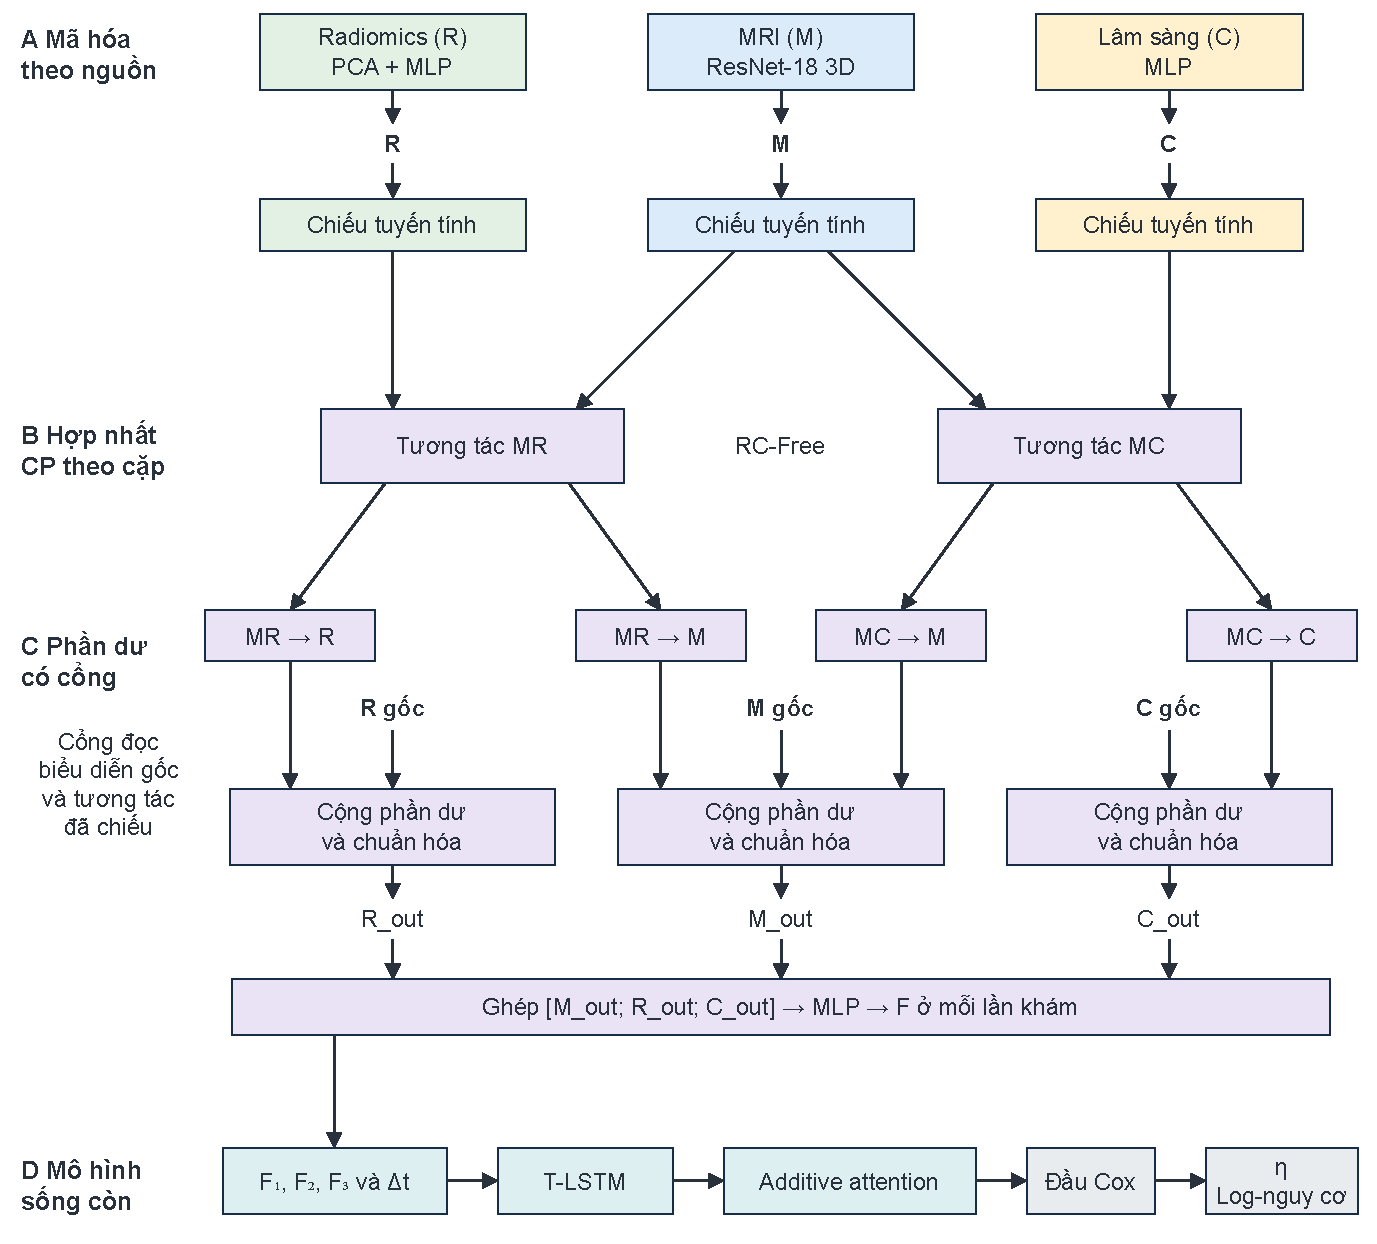
\includegraphics[width=\textwidth]{image/final-pipeline.pdf}
\caption{Sơ đồ quy trình xử lý tổng thể của mô hình RC-Free}
\label{fig:overall}
\end{figure}
\FloatBarrier

Sơ đồ tổng hợp từ dữ liệu dọc đến đánh giá sống còn được trình bày ở Hình~\ref{fig:master-pipeline}, Phụ lục~\ref{app:master-pipeline}.

\section{Thiết kế nghiên cứu và xây dựng dữ liệu}
\label{sec:study-design}

\subsection{Tiêu chí chọn mẫu và ba lần khám}
Dữ liệu nghiên cứu lấy từ Alzheimer's Disease Neuroimaging Initiative (ADNI), một nghiên cứu dọc đa trung tâm về suy giảm nhận thức và AD \cite{weiner2015impact,jack2008adnimri}. Sau khi liên kết mã người tham gia dạng chuỗi (PTID) với mã số người tham gia (RID) trong ADNI, tôi chọn cho mỗi người lần khám ban đầu sớm nhất thuộc ADNI1, ADNIGO hoặc ADNI2 thỏa mãn đồng thời ba điều kiện: có ngày hợp lệ, có mã lần khám \texttt{bl} và có chẩn đoán MCI (mã 2). Ký hiệu $b_i$ là ngày khám ban đầu của người $i$ và $L_i=b_i+18$ tháng lịch là \emph{mốc xét điều kiện chọn mẫu}.

Để giữ nhóm chưa tiến triển trong giai đoạn quan sát, người tham gia bị loại nếu có chẩn đoán AD trong bảng tổng hợp chẩn đoán DXSUM, MMSE $<24$ hoặc CDR-global $\geq1$ tại hoặc trước $L_i$. Sau $L_i$, cần ít nhất một đánh giá MMSE hoặc CDR hợp lệ để xác định biến cố hoặc kiểm duyệt.

Với mỗi người đủ điều kiện, ba ảnh MRI được chọn trong khoảng $[b_i,L_i]$. Việc xếp nhóm bắt đầu từ lần chụp sớm nhất chưa thuộc nhóm nào và gộp vào cùng nhóm các lần chụp tiếp theo trong vòng hai tháng lịch kể từ ngày đó. Trong mỗi nhóm, ảnh chụp chính được ưu tiên hơn ảnh chụp lặp, sau đó mới xét thứ tự hiệu chỉnh ghi trong mô tả ảnh ADNI. Nếu nhiều ảnh cùng mức ưu tiên, ảnh có mã nhỏ nhất được chọn. Khi có hơn ba nhóm, tôi giữ ảnh đầu, ảnh cuối và ảnh trung gian có ngày chụp gần trung điểm thời gian giữa hai ảnh này nhất. Ba ngày chụp thỏa mãn $s_{i1}<s_{i2}<s_{i3}\leq L_i$.

Bảng kiểm soát chất lượng chính thức chưa được liên kết với mã ảnh, nên quy trình dùng nhãn xử lý để xếp thứ tự ưu tiên. Với ADNI1, thứ tự là N3+Scaled+GradWarp+B1, N3+Scaled+GradWarp, N3+Scaled, N3+GradWarp+B1, N3+GradWarp và N3. Với ADNIGO và ADNI2, thứ tự là N3m+GradWarp, N3m, N3+GradWarp và N3. Ảnh không khớp các nhãn trên được xếp sau. B1 biểu thị hiệu chỉnh độ lệch trường tần số vô tuyến, GradWarp biểu thị hiệu chỉnh méo hình học do cuộn chênh từ, N3 và N3m biểu thị hiệu chỉnh bất đồng nhất cường độ, còn Scaled biểu thị chuẩn hóa kích thước theo mẫu đo (phantom).\footnote{Mô tả hiệu chỉnh ảnh của ADNI: \url{https://adni.loni.usc.edu/data-samples/adni-data/neuroimaging/mri/mri-pre-processing/}.} Bảng kê lưu mã ảnh đã chọn cùng thứ tự ưu tiên để có thể truy vết từng lựa chọn.



Hình~\ref{fig:cohort} tóm tắt quá trình lọc từ 899 người có MRI và liên kết định danh thành công xuống 359 người, mỗi người đúng ba MRI, tổng cộng 1077 ảnh. Trong 359 người được chọn, 106 người có biến cố và 253 người bị kiểm duyệt. Xét theo giai đoạn tuyển vào nghiên cứu, 78 người thuộc ADNI1, 80 người thuộc ADNIGO và 201 người thuộc ADNI2.

\begin{figure}[H]
\centering
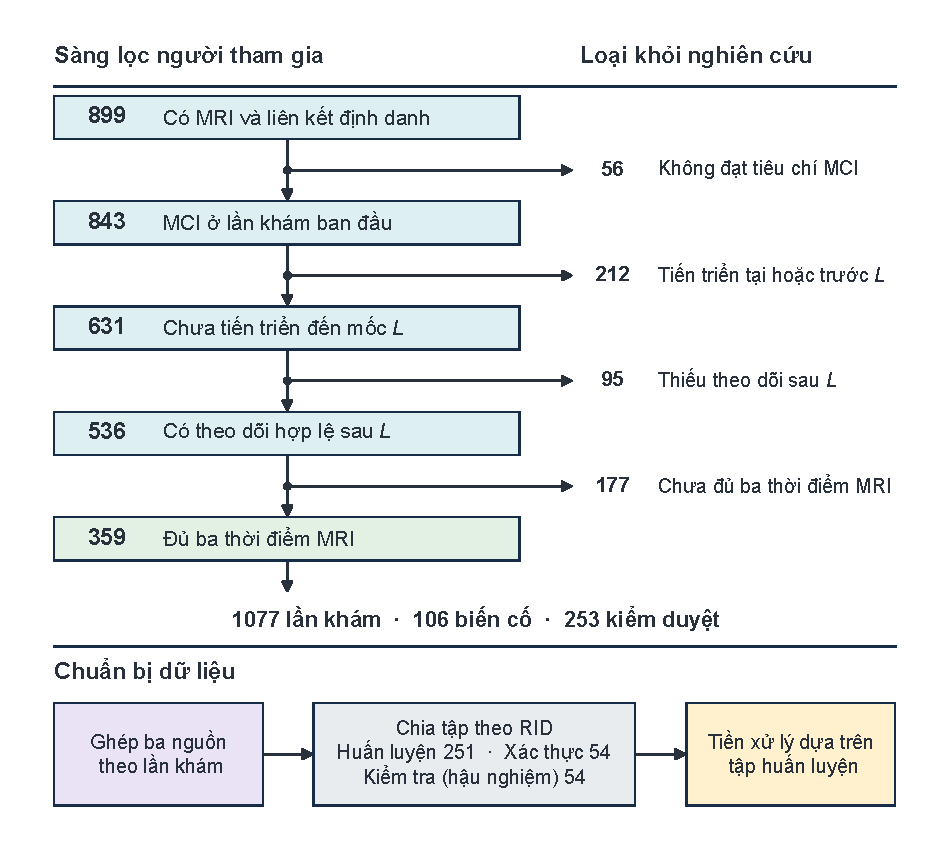
\includegraphics[width=\textwidth]{image/cohort-construction.pdf}
\caption{Quy trình xây dựng và chọn lọc nhóm nghiên cứu dọc}
\label{fig:cohort}
\end{figure}

\subsection{Biến cố, kiểm duyệt và mốc tính thời gian}
Sau mốc chọn mẫu $L_i$, lần đánh giá hợp lệ đầu tiên có MMSE $<24$ hoặc CDR-global $\geq1$ được lấy làm thời điểm ghi nhận biến cố tiến triển. Nếu chưa ghi nhận biến cố, người tham gia được kiểm duyệt tại lần đánh giá MMSE hoặc CDR hợp lệ cuối cùng. Các giá trị thiếu hoặc không hợp lệ không được tính là biến cố.

\Needspace{8\baselineskip}
Thời gian sống còn $t_i$ được tính bằng năm, từ ngày chụp MRI cuối trong ba lần đã chọn ($p_i=s_{i3}$) đến ngày ghi nhận biến cố hoặc kiểm duyệt ($o_i$). Cùng với khoảng thời gian này, chỉ báo $\delta_i$ xác định người tham gia có biến cố (bằng 1) hay bị kiểm duyệt (bằng 0). Hai thành phần của nhãn được tính như sau:
\begin{equation}
 t_i=\frac{o_i-p_i}{365.25},\qquad
 \delta_i=\begin{cases}1,&\text{có biến cố},\\0,&\text{bị kiểm duyệt}.\end{cases}
 \label{eq:survival-target}
\end{equation}

Mốc $L_i$ xác định điều kiện chọn mẫu, còn ngày MRI cuối $p_i$ là gốc tính thời gian sống còn. Trong 359 người, 356 người chụp MRI cuối trước $L_i$ và ba người chụp đúng mốc này. Khoảng cách $L_i-p_i$ có trung vị 186 ngày, khoảng tứ phân vị 169--197 ngày và phạm vi 0--288 ngày. Với những người có $p_i<L_i$, điều kiện chưa tiến triển đến $L_i$ bảo đảm họ không có biến cố trong khoảng từ $p_i$ đến $L_i$. Vì vậy, việc chọn những người này phụ thuộc vào thông tin thu thập sau ngày MRI cuối.

Nếu lấy $p_i$ làm thời điểm dự báo, khoảng theo dõi được bảo đảm không có biến cố có thể gây sai lệch thời gian bất tử (immortal time bias) \cite{suissa2008immortal}.

\subsection{Phân chia dữ liệu và hạn chế rò rỉ thông tin}
\label{sec:data-split}
Tôi chia dữ liệu cố định theo RID để mọi ảnh MRI của một người đều thuộc cùng một tập. Ba tập lần lượt gồm 251 người huấn luyện, 54 người xác thực và 54 người kiểm tra, với số biến cố tương ứng là 74, 16 và 16. Khi ghép các nguồn theo mã người, lần khám, mã ảnh và tập dữ liệu, mỗi lần khám phải có duy nhất một kết quả khớp giữa các nguồn. Chỉ dữ liệu huấn luyện được dùng để xác định cách điền dữ liệu thiếu, ước lượng tham số chuẩn hóa, nhận diện đặc trưng hằng và học PCA. Các biến dự báo không bao gồm chẩn đoán, trạng thái biến cố, ngày kết cục và thời gian sống còn.

Mỗi ảnh MRI được ghép với lần đánh giá lâm sàng hợp lệ gần nhất của cùng người trong cửa sổ $\pm90$ ngày. Nếu hai bản ghi cách đều ngày chụp, thứ tự ưu tiên là ngày đánh giá sớm hơn, rồi đến mã bản ghi nhỏ hơn. Trong 359 người, 57 người có điểm MMSE hoặc CDR lấy từ số đo sau ngày MRI cuối $p_i$. Ba lượt ghép MMSE và ba lượt ghép CDR sử dụng số đo sau cả mốc chọn mẫu $L_i$. Mặc dù tất cả các số đo này đều có trước ngày kết cục $o_i$, những số đo thu thập sau ngày MRI cuối $p_i$ vẫn là thông tin tương lai nếu lấy ngày chụp này làm mốc dự báo.

Để mô tả thành phần của ba tập dữ liệu, Bảng~\ref{tab:baseline-characteristics} tổng hợp đặc điểm của người tham gia tại lần chụp MRI đầu tiên, phân theo từng tập và tình trạng ghi nhận biến cố tiến triển.

Các kiểm định so sánh tuổi, học vấn và khoảng cách giữa các lần chụp ở ba tập đều cho $p>0.05$. Trung vị thời gian từ MRI cuối đến kết cục lần lượt là 3.07 năm ở tập huấn luyện, 3.84 năm ở tập xác thực và 3.25 năm ở tập kiểm tra. Khoảng tứ phân vị tương ứng là [1.98; 6.65], [1.99; 5.90] và [1.66; 6.86] năm. Thời gian theo dõi dài nhất ở tập xác thực (18.26 năm) vượt thời gian dài nhất ở tập huấn luyện (13.95 năm). Mục~\ref{sec:survival-evaluation} trình bày cách xử lý chênh lệch này khi tính AUC.

Tại lần MRI đầu, 132 người có điểm MMSE hợp lệ và 131 người có điểm CDR hợp lệ. Xét riêng từng thang MMSE và CDR, 227 người có bản ghi gần nhất nằm ngoài cửa sổ $\pm90$ ngày quanh lần chụp này (khoảng cách trung vị 102 ngày). Riêng CDR có thêm một người có bản ghi trong cửa sổ nhưng giá trị không hợp lệ. Ngày chụp MRI đầu và ngày khám ban đầu cách nhau trung vị 71 ngày. Mục~\ref{sec:preprocessing} trình bày cách điền giá trị thiếu bằng trung vị huấn luyện và cách mã hóa tình trạng quan sát của từng biến.

\begin{landscape}
\begin{table}[p]
\centering\small
\caption[Đặc điểm người tham gia tại MRI đầu]{Đặc điểm người tham gia tại MRI đầu, chia theo tập và trạng thái kết cục.}
\label{tab:baseline-characteristics}
\setlength{\tabcolsep}{4pt}
\begin{tabular}{@{}lrrrrrrr@{}}
\toprule
& \multicolumn{2}{c}{Huấn luyện ($N=251$)} & \multicolumn{2}{c}{Xác thực ($N=54$)} & \multicolumn{2}{c}{Kiểm tra ($N=54$)} & $p$ \\
\cmidrule(lr){2-3}\cmidrule(lr){4-5}\cmidrule(lr){6-7}
Đặc điểm & $\delta=0$ & $\delta=1$ & $\delta=0$ & $\delta=1$ & $\delta=0$ & $\delta=1$ & \\
\midrule
Số người & 177 & 74 & 38 & 16 & 38 & 16 & -- \\
Tuổi tại MRI đầu (năm) & $71.64 \pm 7.54$ & $73.41 \pm 7.17$ & $71.29 \pm 8.64$ & $74.86 \pm 5.64$ & $70.03 \pm 7.58$ & $72.74 \pm 6.72$ & 0.489 \\
Nam, n (\%) & 96 (54.24) & 49 (66.22) & 23 (60.53) & 10 (62.50) & 28 (73.68) & 9 (56.25) & 0.337 \\
Học vấn (năm) & $16.37 \pm 2.72$ & $16.61 \pm 2.58$ & $15.32 \pm 2.57$ & $17.00 \pm 2.53$ & $17.00 \pm 2.63$ & $16.19 \pm 2.95$ & 0.147 \\
MMSE ban đầu & $28.57 \pm 1.38$ (53) & $27.22 \pm 1.77$ (36) & $28.54 \pm 1.13$ (13) & $27.75 \pm 1.49$ (8) & $28.25 \pm 1.53$ (16) & $26.83 \pm 2.04$ (6) & 0.869 \\
CDR-global ban đầu & $0.44 \pm 0.16$ (52) & $0.49 \pm 0.08$ (36) & $0.38 \pm 0.22$ (13) & $0.44 \pm 0.18$ (8) & $0.47 \pm 0.12$ (16) & $0.50 \pm 0.00$ (6) & 0.206 \\
CDR-SB ban đầu & $0.92 \pm 0.57$ (52) & $1.68 \pm 0.96$ (36) & $1.04 \pm 0.80$ (13) & $1.56 \pm 1.15$ (8) & $1.28 \pm 0.91$ (16) & $1.67 \pm 0.93$ (6) & 0.726 \\
$s_2-s_1$ (ngày) & $120.47 \pm 40.57$ & $134.04 \pm 45.02$ & $131.76 \pm 41.84$ & $129.50 \pm 46.47$ & $124.34 \pm 42.45$ & $137.50 \pm 44.46$ & 0.431 \\
$s_3-s_1$ (ngày) & $305.12 \pm 44.16$ & $313.04 \pm 42.83$ & $307.32 \pm 34.03$ & $312.19 \pm 75.38$ & $312.08 \pm 55.05$ & $315.50 \pm 38.44$ & 0.890 \\
$t_i$ (năm), TB $\pm$ SD & $5.11 \pm 3.91$ & $3.41 \pm 2.79$ & $5.59 \pm 4.73$ & $3.85 \pm 3.21$ & $5.51 \pm 4.34$ & $3.11 \pm 2.54$ & 0.871 \\
$t_i$ (năm), trung vị [Q1; Q3] & 3.64 [2.02; 7.54] & 2.09 [1.66; 4.42] & 3.92 [2.05; 6.73] & 3.69 [1.44; 4.88] & 4.06 [2.02; 8.20] & 2.42 [1.54; 3.64] & -- \\
\bottomrule
\end{tabular}
\par\vspace{6pt}
\begin{minipage}{0.96\linewidth}\small
$\delta=0$ biểu thị kiểm duyệt và $\delta=1$ biểu thị biến cố. Trừ các dòng có ghi riêng, bảng trình bày trung bình $\pm$ SD mẫu. Với MMSE và CDR, số trong ngoặc là số quan sát hợp lệ trước khi điền thiếu. Tỷ lệ nam tính trên số người có thông tin giới tính. Tuổi được ước tính từ tháng và năm sinh, quy ước ngày sinh là ngày 15. Các biến nhân khẩu học lấy từ bản ghi hợp lệ gần MRI đầu nhất, tính đến ngày chụp. Các điểm MMSE và CDR được ghép trong cửa sổ $\pm90$ ngày. Giá trị $p$ mô tả khác biệt giữa ba tập, gộp cả hai trạng thái kết cục, theo kiểm định Kruskal--Wallis cho biến định lượng và kiểm định $\chi^2$ cho giới tính. $s_3-s_1$ là khoảng thời gian từ MRI đầu đến MRI cuối. $t_i$ là thời gian từ MRI cuối đến biến cố hoặc kiểm duyệt.
\end{minipage}
\end{table}
\end{landscape}


\subsection{Phạm vi đánh giá và diễn giải}
\label{sec:evaluation-scope}
Phạm vi đánh giá khả năng xếp hạng nguy cơ giới hạn trong nhóm hồi cứu gồm những người có đủ ba MRI và chưa tiến triển theo tiêu chí chọn mẫu tại $L_i$.

Tôi dùng tập xác thực để chọn mô hình và báo cáo kết quả chính. Do tập kiểm tra cũng đã được sử dụng trong quá trình phát triển, kết quả trên tập này là đánh giá hậu nghiệm (post-hoc). Điểm nguy cơ tương đối do mô hình Cox ước lượng được dùng để xếp hạng cá thể, so sánh các nhóm nguy cơ và đánh giá khả năng phân biệt tại từng mốc thời gian. Việc chuyển điểm này thành xác suất biến cố cá nhân đòi hỏi ước lượng thêm hàm nguy cơ tích lũy nền $H_0(t)$.

\section{Tiền xử lý và biểu diễn từng nguồn dữ liệu}
\label{sec:preprocessing}

\subsection{Minh họa ba nguồn dữ liệu đầu vào}
Hình~\ref{fig:input-three-sources} minh họa ba dạng thông tin được liên kết tại mỗi lần khám. Ảnh MRI, các số đo radiomics và điểm MMSE/CDR lần lượt đi qua ba bộ mã hóa riêng để tạo vectơ đặc trưng cho từng nguồn.

\begin{figure}[H]
\centering
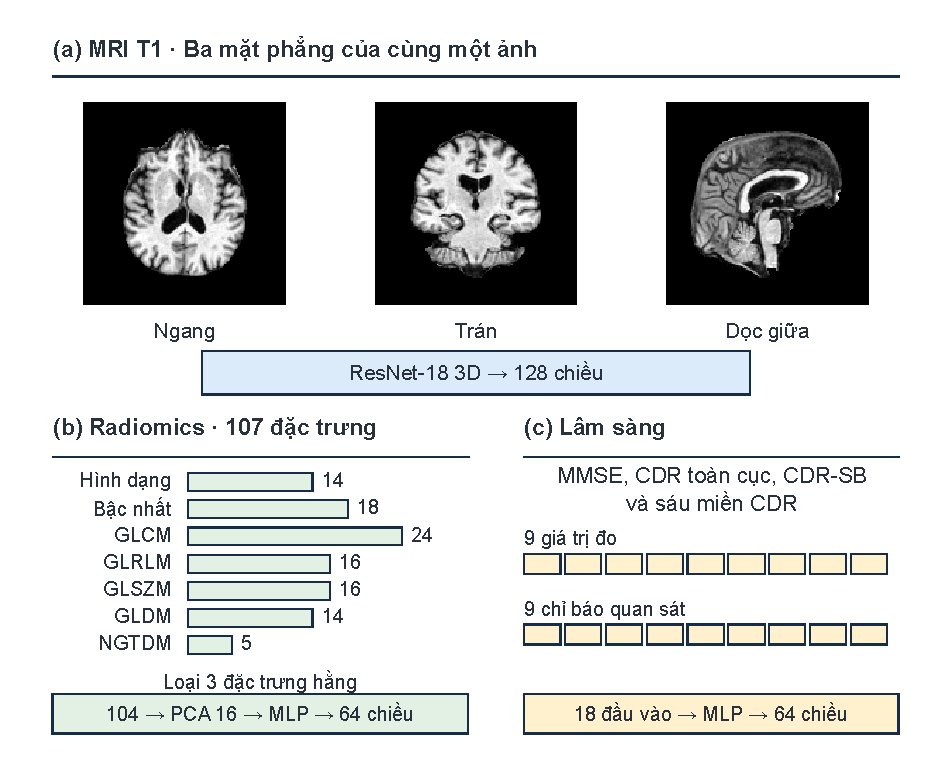
\includegraphics[width=\textwidth]{image/input-three-sources.pdf}
\caption{Minh họa ba nguồn dữ liệu đầu vào và các biểu diễn đặc trưng}
\label{fig:input-three-sources}
\end{figure}






\subsection{MRI và bộ mã hóa dùng chung}
Mỗi người tham gia có ba ảnh cộng hưởng từ có trọng số T1 (MRI T1-weighted), ghi nhận cấu trúc não ở ba lần khám. Ngay cả khi hình dạng một cấu trúc chưa thay đổi, vị trí của nó trên ảnh vẫn có thể khác giữa hai lần chụp. Chẳng hạn, nếu người tham gia hơi nghiêng đầu ở lần chụp thứ hai, hồi hải mã trái có thể xuất hiện ở vị trí khác so với lần đầu. Khi đối chiếu hai ảnh, độ lệch do tư thế đầu dễ bị nhầm với thay đổi hình thái mà mô hình cần khai thác, chẳng hạn như teo hồi hải mã hoặc giãn não thất. Vì vậy, tôi đưa ba ảnh về cùng hệ tọa độ và lưới lấy mẫu, đồng thời chuẩn hóa thang cường độ riêng cho từng ảnh. Hình~\ref{fig:mri-preprocessing} tóm tắt quy trình từ ba lần chụp đến đầu vào của nhánh ảnh.

\begin{figure}[H]
\centering
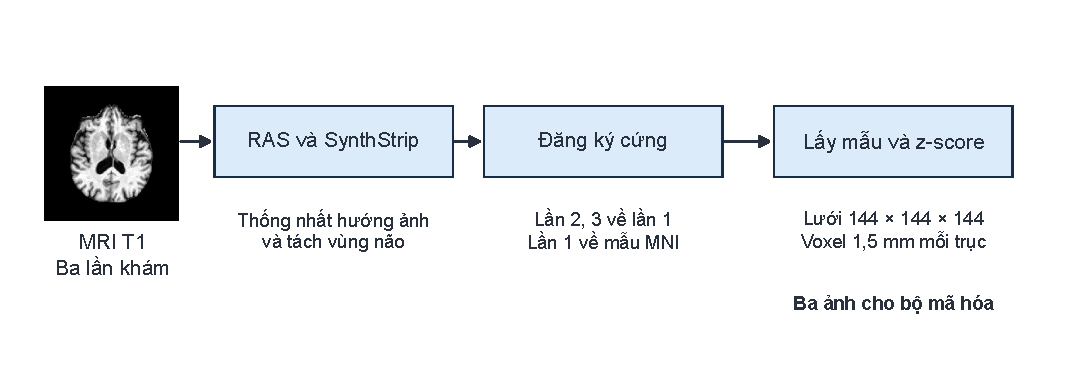
\includegraphics[width=\textwidth]{image/mri-preprocessing.pdf}
\caption{Quy trình tiền xử lý chuỗi ảnh MRI T1 dọc}
\label{fig:mri-preprocessing}
\end{figure}

\noindent\textbf{Chuẩn hóa hướng ảnh và tách não.}
Mỗi ảnh MRI là một khối dữ liệu ba chiều. Mỗi phần tử, gọi là voxel, mang một giá trị cường độ tại một vị trí trên lưới. Do các ảnh có thể được lưu theo những quy ước hướng khác nhau, trước tiên tôi đưa chúng về quy ước RAS (\emph{Right--Anterior--Superior}). Theo quy ước này, ba chiều dương lần lượt hướng về bên phải, phía trước và phía trên của người được chụp. Sau bước này, các trục có cùng ý nghĩa giải phẫu, nhưng tư thế đầu giữa các lần chụp vẫn có thể khác nhau.

Trên ảnh có cả não, hộp sọ, da đầu và các mô xung quanh. Tôi dùng SynthStrip, một phương pháp học sâu, để xác định vùng não cần giữ lại \cite{hoopes2022synthstrip}. Kết quả là một mặt nạ não (\emph{brain mask}) có cùng vị trí không gian với ảnh: voxel mang giá trị 1 thuộc vùng cần giữ, còn voxel mang giá trị 0 nằm ngoài vùng đó. Mặt nạ xác định phạm vi lấy số liệu cho bước chuẩn hóa cường độ. Đây là mặt nạ chung của vùng não, không phân biệt riêng chất xám, chất trắng hay dịch não tủy.

\noindent\textbf{Căn chỉnh giữa các lần khám.}
Tôi chọn ảnh MRI đầu tiên của mỗi người làm ảnh tham chiếu, rồi căn chỉnh riêng ảnh thứ hai và ảnh thứ ba về ảnh đầu bằng phép đăng ký cứng (\emph{rigid registration}). Phép biến đổi này có sáu bậc tự do: ba phép tịnh tiến dọc theo các trục không gian và ba phép quay quanh các trục đó. Nếu ở lần chụp thứ hai đầu vừa dịch sang bên vừa nghiêng, thành phần tịnh tiến điều chỉnh độ lệch vị trí, còn thành phần quay điều chỉnh góc nghiêng. Với một điểm có tọa độ $\mathbf{x}$ trong ảnh cần căn chỉnh, tọa độ tương ứng $\mathbf{x}'$ trong hệ tham chiếu được biểu diễn bởi
\[
 \mathbf{x}'=\mathbf{R}\mathbf{x}+\mathbf{t},
\]
trong đó $\mathbf{R}$ là ma trận quay và $\mathbf{t}$ là vectơ tịnh tiến. Cùng một phép quay và tịnh tiến tác động lên toàn bộ ảnh nên khoảng cách giữa hai điểm bất kỳ trong ảnh được bảo toàn. Nhờ đó, có thể đối chiếu vị trí hồi hải mã hay não thất giữa các lần chụp mà phép căn chỉnh không co giãn từng cấu trúc để ép chúng trùng khớp.

\noindent\textbf{Đưa chuỗi ảnh về hệ tọa độ MNI.}
Sau khi hai ảnh chụp sau đã có mốc tham chiếu là ảnh đầu, mỗi người vẫn có một mốc riêng. Để các chuỗi ảnh của nhiều người có chung hệ tọa độ, tôi căn chỉnh ảnh đầu của từng người về mẫu não tham chiếu MNI152NLin2009cAsym, cũng bằng phép đăng ký cứng sáu bậc tự do. Hình~\ref{fig:mri-registration} minh họa quan hệ giữa hai bước. Đối với một điểm trên ảnh lần hai, vị trí của nó được quy chiếu về ảnh lần đầu, rồi từ hệ tọa độ của ảnh lần đầu sang hệ tọa độ MNI. Quan hệ này cũng áp dụng cho ảnh lần ba. Như vậy, ảnh đầu làm mốc so sánh giữa các lần khám của một người, còn mẫu MNI làm mốc chung giữa những người tham gia.

\begin{figure}[H]
\centering
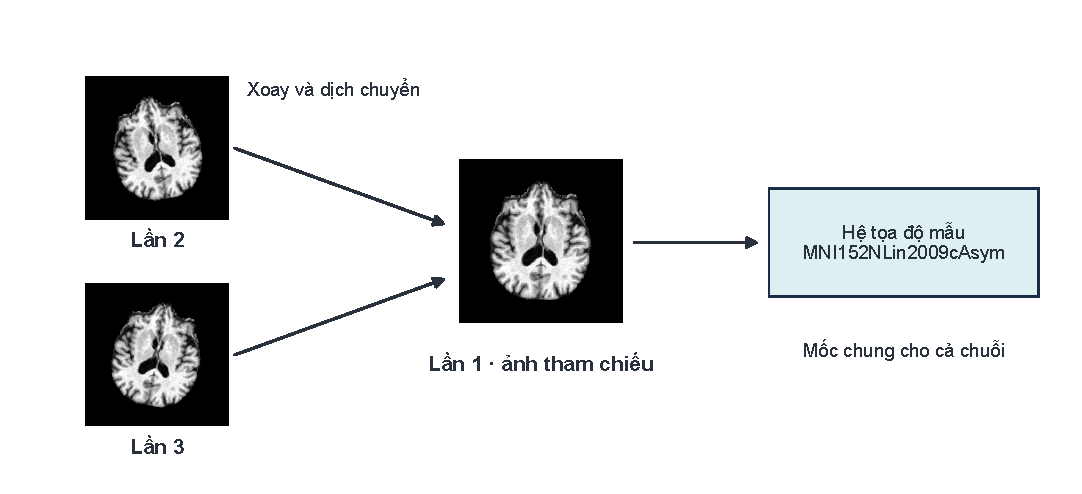
\includegraphics[width=\textwidth]{image/mri-registration.pdf}
\caption{Quy trình căn chỉnh không gian MRI giữa các lần khám và về mẫu MNI}
\label{fig:mri-registration}
\end{figure}

Phép đăng ký cứng giữ nguyên hình dạng và kích thước hình học của não. Quy trình không dùng biến đổi affine có thành phần co giãn hoặc biến dạng xiên, cũng không dùng đăng ký phi tuyến để làm biến dạng cục bộ. Lựa chọn này giới hạn những thay đổi hình học do bước căn chỉnh đưa vào ảnh. Vì hình dạng não tự nhiên khác nhau giữa các cá thể, việc dùng chung hệ tọa độ MNI không bảo đảm ranh giới của mọi cấu trúc giải phẫu đều trùng nhau giữa hai người.

\noindent\textbf{Lấy mẫu lại ảnh và mặt nạ.}
Sau căn chỉnh, ba ảnh của mỗi người được biểu diễn trên một lưới chung $144\times144\times144$ voxel. Kích thước voxel là 1.5~mm theo cả ba trục, tức là khoảng cách giữa tâm hai voxel kề nhau dọc một trục bằng 1.5~mm. Khi lấy mẫu lại (\emph{resampling}), tâm voxel trên lưới mới có thể nằm giữa các vị trí đã lấy mẫu trên ảnh ban đầu. Đối với ảnh MRI, tôi dùng nội suy tuyến tính để ước lượng cường độ từ các voxel lân cận. Chẳng hạn, trong ví dụ một chiều, nếu hai vị trí liền kề có cường độ 100 và 200 thì giá trị nội suy ở chính giữa là 150.

Với mặt nạ nhị phân, nội suy như vậy có thể tạo ra giá trị nằm giữa 0 và 1, làm mất ý nghĩa của nhãn vùng não. Thay vào đó, tôi dùng nội suy láng giềng gần nhất (\emph{nearest-neighbor interpolation}): mỗi voxel trên lưới mới nhận nhãn của voxel nguồn gần nhất. Nhờ vậy, ảnh và mặt nạ cùng nằm trên lưới đầu ra, còn mặt nạ vẫn chỉ nhận giá trị 0 hoặc 1.

\noindent\textbf{Chuẩn hóa cường độ trong vùng não.}
Cường độ MRI T1 mang tính tương đối: cùng một loại mô có thể cho giá trị khác nhau giữa hai lần chụp do thiết bị hoặc thiết lập thu nhận. Để giảm khác biệt về thang cường độ, tôi chuẩn hóa z-score riêng cho từng ảnh. Gọi $I(v)$ là cường độ tại voxel $v$ bên trong mặt nạ, còn $\mu$ và $\sigma$ lần lượt là trung bình và độ lệch chuẩn tính trên tất cả các voxel thuộc mặt nạ của chính ảnh đó. Với $\sigma>0$, cường độ sau chuẩn hóa là
\[
 z(v)=\frac{I(v)-\mu}{\sigma}.
\]
Chẳng hạn, nếu $\mu=100$, $\sigma=20$ và $I(v)=130$ thì $z(v)=(130-100)/20=1.5$. Giá trị này cho biết cường độ tại voxel đang xét cao hơn trung bình trong vùng não của ảnh 1.5 độ lệch chuẩn. Sau chuẩn hóa, cường độ trong mặt nạ có trung bình bằng 0 và độ lệch chuẩn bằng 1. Các voxel ngoài mặt nạ không tham gia tính hai thống kê này và được đặt bằng 0 ở ảnh đầu ra.

Tóm lại, bước chuẩn hóa z-score chỉ đồng nhất thang đo độ sáng tối giữa các ảnh chụp khác nhau mà hoàn toàn không làm thay đổi vị trí hay hình học của các voxel trong não. Trong quy trình này, tôi không áp dụng thêm bước khử nhiễu từ trường N4 (\emph{N4 bias field correction} — một kỹ thuật thường dùng để làm phẳng độ chênh lệch ánh sáng cục bộ do cuộn cảm máy chụp), nhằm tránh làm biến dạng độ tương phản mô tự nhiên của ảnh gốc. 

Như vậy, sau toàn bộ chuỗi tiền xử lý từ tách não, căn chỉnh tọa độ cho đến chuẩn hóa cường độ, bộ mã hóa sẽ tiếp nhận ba khối ảnh MRI đã được đưa về cùng một chuẩn thống nhất: cùng kích thước lưới $144\times144\times144$, cùng hệ tọa độ giải phẫu MNI, và cùng một thang đo giá trị. Nhờ loại bỏ được các yếu tố gây nhiễu ngoại cảnh như tư thế nghiêng đầu của người bệnh hay sự khác biệt về cài đặt máy chụp giữa các lần tái khám, mô hình học sâu có thể tập trung tối đa vào việc trích xuất những biến đổi giải phẫu bệnh lý thực sự — đặc biệt là hiện tượng teo mô não và giãn rộng não thất — diễn ra qua ba lần khám.

Sau tiền xử lý, cả ba MRI dùng chung bộ mã hóa ResNet-18 3D triển khai bằng MONAI, khởi tạo từ trọng số MedicalNet; sau đây gọi ngắn là ResNet-18 3D \cite{he2016deep,cardoso2022monai}. Mỗi tầng trong bốn tầng của mạng có hai khối cơ bản (BasicBlock), mỗi khối gồm hai phép tích chập với nhân $3^3$, chuẩn hóa BatchNorm, hàm kích hoạt ReLU và đường nối phần dư \cite{ioffe2015batchnorm,nair2010rectified}. Số kênh của bốn tầng lần lượt là 64, 128, 256 và 512. Sau gộp toàn cục, vectơ 512 chiều qua lớp tuyến tính $512\to128$, GELU, Dropout 0.20 và LayerNorm để tạo $M$ \cite{hendrycks2016gelu,srivastava2014dropout,ba2016layernorm}. Khi khởi tạo bộ mã hóa bằng trọng số MedicalNet từ Med3D \cite{chen2019med3d}, tôi nạp đầy đủ trọng số và trạng thái BatchNorm của mạng trích xuất đặc trưng, đồng thời bỏ khối đầu ra tiền huấn luyện. Toàn mạng được tinh chỉnh ngay từ vòng huấn luyện đầu tiên.

Bảng~\ref{tab:mri-encoder-shapes} trình bày kích thước bản đồ đặc trưng theo cấu hình MONAI (phiên bản 1.5.2)\footnote{Mã nguồn phiên bản: \url{https://github.com/Project-MONAI/MONAI/blob/1.5.2/monai/networks/nets/resnet.py}.}. Mỗi bản đồ đặc trưng có dạng $[B,C_{\mathrm{ch}},D,H,W]$, trong đó $B$ là cỡ lô, $C_{\mathrm{ch}}$ là số kênh và $D,H,W$ là ba kích thước không gian. Ký hiệu $C$ dùng riêng cho nhánh lâm sàng. Cả ba lần khám dùng chung bộ mã hóa. Sau bước gộp, các vectơ được xếp thành chuỗi $[B,T,F]$ trước phép chiếu, với $T=3$ là số lần khám và $F$ là số chiều đặc trưng.

\begin{table}[H]
\centering
\small
\caption{Kích thước đặc trưng trong bộ mã hóa MRI}
\label{tab:mri-encoder-shapes}
\begin{tabularx}{\textwidth}{@{}Y l@{}}
\toprule
\textbf{Bước} & \textbf{Kích thước đầu ra} \\
\midrule
MRI đầu vào & $[B,1,144,144,144]$ \\
Tích chập $7^3$, bước 1, đệm 3; BN; ReLU & $[B,64,144,144,144]$ \\
Gộp cực đại $3^3$, bước 2, đệm 1 & $[B,64,72,72,72]$ \\
Tầng ResNet 1: hai khối cơ bản & $[B,64,72,72,72]$ \\
Tầng 2: khối đầu có bước 2 & $[B,128,36,36,36]$ \\
Tầng 3: khối đầu có bước 2 & $[B,256,18,18,18]$ \\
Tầng 4: khối đầu có bước 2 & $[B,512,9,9,9]$ \\
Gộp trung bình toàn cục; trải phẳng & $[B,512,1,1,1]\to[B,512]$ \\
Xếp ba vectơ sau gộp & $[B,3,512]$ \\
Tuyến tính; GELU; Dropout; LayerNorm & $[B,3,128]$ \\
\bottomrule
\end{tabularx}
\end{table}

\subsection{Radiomics}
\label{sec:radiomics-pipeline}

Bên cạnh bộ mã hóa CNN học sâu — vốn trích xuất các biểu diễn ẩn trừu tượng từ ảnh khối 3D — tôi xây dựng một nhánh xử lý song song dựa trên \emph{Radiomics} để khai thác các đặc trưng hình học và kết cấu mô não được định nghĩa toán học tường minh \cite{vangriethuysen2017computational}. Trong khi mạng nơ-ron sâu thường hoạt động như một ``hộp đen'', các chỉ số radiomics mang ý nghĩa y sinh cụ thể, cho phép định lượng trực tiếp mức độ teo thoái hóa hình thái cũng như sự biến đổi vi mô về mật độ mô não của người bệnh.

\noindent\textbf{Trích xuất đặc trưng bằng PyRadiomics.}
Từ ảnh MRI đã qua tiền xử lý cùng mặt nạ não (\emph{brain mask}), tôi sử dụng thư viện chuẩn hóa PyRadiomics để trích xuất 107 đặc trưng định lượng thuộc bảy nhóm khác nhau (Bảng~\ref{tab:radiomics-groups}). Các nhóm này bao gồm:
\begin{itemize}
\item \emph{Đặc trưng hình dạng} (14 biến): Đo lường kích thước hình học tổng thể của vùng não, chẳng hạn như thể tích não thật (\emph{MeshVolume}) và diện tích bề mặt (\emph{SurfaceArea}).
\item \emph{Thống kê cường độ bậc nhất} (18 biến): Mô tả phân bố độ sáng tối của các voxel trong não mà không xét đến vị trí không gian, ví dụ như giá trị trung bình (\emph{Mean}), độ lệch chuẩn, độ bất đối xứng (\emph{Skewness}) và độ hỗn loạn (\emph{Entropy}).
\item \emph{Các nhóm kết cấu không gian} (75 biến): Nắm bắt mối tương quan không gian và độ thô mịn giữa các voxel lân cận thông qua các ma trận toán học kinh điển, bao gồm ma trận đồng xuất hiện mức xám (GLCM, 24 biến), ma trận độ dài dải mức xám (GLRLM, 16 biến), ma trận kích thước vùng mức xám (GLSZM, 16 biến), ma trận phụ thuộc mức xám (GLDM, 14 biến) và ma trận chênh lệch độ xám theo vùng lân cận (NGTDM, 5 biến).
\end{itemize}

\noindent\textbf{Chuẩn hóa cường độ riêng cho Radiomics.}
Một điểm kỹ thuật then chốt cần phân biệt rõ là sự khác biệt về yêu cầu đầu vào giữa nhánh CNN và nhánh Radiomics:
\begin{itemize}
\item \emph{Nhánh CNN (ResNet-18 3D)} tiếp nhận ảnh đã qua chuẩn hóa z-score (trung bình 0, độ lệch chuẩn 1), vì đây là dạng phân phối tối ưu giúp gradient lan truyền ổn định trong các mạng nơ-ron sâu.
\item \emph{Nhánh Radiomics} lại đòi hỏi một cách tiếp cận khác: các thuật toán tính ma trận kết cấu (như GLCM hay GLSZM) bắt buộc phải chia dải cường độ của ảnh thành một số lượng mức xám rời rạc cố định (\texttt{binCount=64}). Để các mức xám này có cùng khoảng chia và giữ đúng ý nghĩa vật lý giữa các bệnh nhân khác nhau, toàn bộ cường độ voxel trong mặt nạ trước hết được co giãn Min-Max tuyến tính về khoảng $[0, 1]$ (voxel tối nhất bằng 0, sáng nhất bằng 1). Nếu dùng ảnh z-score (vốn có cả giá trị âm lẫn dương và biên độ biến thiên không bị chặn), việc chia 64 mức xám sẽ bị xáo trộn giữa các lần chụp, dẫn đến các phép đo kết cấu bị sai lệch.
\end{itemize}

\noindent\textbf{Lọc biến hằng và giảm chiều bằng PCA.}
Do toàn bộ voxel trong não đã được chuẩn hóa về dải $[0, 1]$, ba đặc trưng thống kê bậc nhất — bao gồm giá trị cường độ nhỏ nhất (luôn bằng 0), giá trị lớn nhất (luôn bằng 1) và khoảng biến thiên cường độ (luôn bằng $1-0=1$) — trở thành các giá trị hằng số giống hệt nhau ở mọi người tham gia. Vì không chứa thông tin phân biệt bệnh lý, ba biến này được loại bỏ, giữ lại chính xác 104 đặc trưng thực sự hữu ích.

Trong số 104 đặc trưng còn lại, nhiều biến có mức độ tương quan chéo cao (chẳng hạn các đặc trưng đo kích thước não hoặc các chỉ số đồng nhất kết cấu). Để loại bỏ hiện tượng đa cộng tuyến và tránh bùng nổ tham số khi kết hợp với các nguồn dữ liệu khác, tôi áp dụng Phân tích thành phần chính (PCA) \cite{jolliffe2016pca}. Nhằm triệt tiêu hoàn toàn nguy cơ rò rỉ dữ liệu, các tham số chuẩn hóa z-score của từng đặc trưng và ma trận chuyển đổi PCA đều được ước lượng nghiêm ngặt trên tập huấn luyện, sau đó mới áp dụng cố định cho tập xác thực và kiểm tra. Với ngưỡng giữ lại ít nhất 99\% tổng phương sai, mô hình xác định được đúng 16 thành phần chính tại mỗi lần khám.

\noindent\textbf{Tạo biểu diễn nhúng qua mạng MLP.}
Cuối cùng, vectơ 16 chiều sau PCA được đưa qua một khối mạng perceptron đa tầng ($16 \to 128 \to 64$) gồm kích hoạt phi tuyến GELU, tỉ lệ Dropout 0.20 và lớp chuẩn hóa LayerNorm \cite{hendrycks2016gelu,srivastava2014dropout,ba2016layernorm}. Đầu ra của khối này là một vectơ biểu diễn Radiomics $R \in \mathbb R^{64}$, vừa cô đọng các dấu hiệu giải phẫu vi mô, vừa đồng bộ kích thước để sẵn sàng tham gia vào các tầng hợp nhất đa phương thức tiếp theo.

\begin{table}[H]
\centering\small
\caption[Các nhóm đặc trưng radiomics]{Bảy nhóm đặc trưng radiomics trích từ ảnh và mặt nạ toàn não. Cột cuối nêu ví dụ thuộc từng nhóm.}
\label{tab:radiomics-groups}
\begin{tabularx}{\linewidth}{@{}L{2.7cm}r Y Y@{}}
\toprule
Nhóm & Số lượng & Thông tin mô tả & Ví dụ \\
\midrule
Hình dạng & 14 & Hình học của mặt nạ não & Thể tích (MeshVolume), diện tích bề mặt (SurfaceArea) \\
Thống kê bậc nhất & 18 & Phân bố cường độ trong mặt nạ & Trung bình (Mean), phương sai (Variance), Entropy \\
GLCM & 24 & Quan hệ mức xám giữa các cặp voxel & Contrast, Correlation \\
GLRLM & 16 & Độ dài chuỗi voxel cùng mức xám theo hướng & ShortRunEmphasis, LongRunEmphasis \\
GLSZM & 16 & Kích thước vùng liên thông cùng mức xám & SmallAreaEmphasis, LargeAreaEmphasis \\
GLDM & 14 & Mức phụ thuộc cường độ giữa voxel và lân cận & DependenceEntropy, DependenceVariance \\
NGTDM & 5 & Chênh lệch cường độ với lân cận & Coarseness, Contrast, Busyness, Complexity, Strength \\
\midrule
Tổng & 107 & Còn 104 sau khi loại Maximum, Minimum và Range & PCA giữ 16 thành phần \\
\bottomrule
\end{tabularx}
\end{table}


\subsection{Dữ liệu lâm sàng và chỉ báo có dữ liệu}
Trong chín biến dự báo của nhánh lâm sàng, ba biến tổng hợp gồm MMSE-total, CDR-global và tổng điểm các miền CDR (CDR-sum-of-boxes, CDR-SB). Sáu biến còn lại là điểm của từng miền CDR, bao gồm trí nhớ, định hướng, phán đoán, hoạt động cộng đồng, sinh hoạt gia đình và sở thích, cùng khả năng tự chăm sóc \cite{folstein1975mmse,morris1993cdr}. Tôi điền mỗi giá trị thiếu bằng trung vị của biến tại lần khám tương ứng trên tập huấn luyện. Nếu toàn bộ số đo của biến đều thiếu ở lần khám đó, tôi dùng trung vị của biến trên toàn tập huấn luyện. Sau khi điền thiếu, tôi chuẩn hóa các giá trị theo trung bình và độ lệch chuẩn ước lượng từ tập huấn luyện. Để mô hình phân biệt số đo thực tế với giá trị được điền thay, mỗi biến có một chỉ báo nhị phân bằng 1 nếu có số đo và bằng 0 nếu thiếu trước khi điền. Nhờ kết hợp chín giá trị lâm sàng với chín chỉ báo tương ứng, nhánh lâm sàng có đầu vào 18 chiều để đưa qua MLP $18\to64\to64$ với GELU, Dropout 0.10 và LayerNorm, tạo biểu diễn lâm sàng $C\in\mathbb R^{64}$.

Bảng~\ref{tab:clinical-inputs} liệt kê từng biến để phân biệt chín giá trị lâm sàng với chín chỉ báo dữ liệu thiếu. CDR-global và CDR-SB là hai cách tổng hợp khác nhau; sáu miền CDR vẫn được giữ riêng để mô hình nhận thông tin cụ thể của từng hoạt động.
\begin{table}[H]
\centering\small
\caption[Chín biến lâm sàng đầu vào]{Chín giá trị trước khi chuẩn hóa, theo đúng thứ tự đầu vào của mô hình. Mỗi giá trị có thêm một chỉ báo quan sát tương ứng.}
\label{tab:clinical-inputs}
\begin{tabularx}{\linewidth}{@{}r L{3.6cm}Y@{}}
\toprule
Vị trí & Biến lâm sàng & Ý nghĩa \\
\midrule
1 & MMSE-total & Tổng điểm đánh giá nhận thức, thang 0--30 \\
2 & CDR-global & Mức độ suy giảm nhận thức và chức năng tổng thể \\
3 & CDR-SB & Tổng điểm của sáu miền CDR, thang 0--18 \\
4 & CDR: trí nhớ & Khả năng ghi nhớ và nhớ lại thông tin \\
5 & CDR: định hướng & Nhận biết thời gian, địa điểm và hoàn cảnh \\
6 & CDR: phán đoán & Khả năng phán đoán và giải quyết vấn đề \\
7 & CDR: cộng đồng & Khả năng tham gia hoạt động ngoài gia đình \\
8 & CDR: gia đình/sở thích & Khả năng thực hiện công việc tại nhà và duy trì sở thích \\
9 & CDR: tự chăm sóc & Mức độc lập trong chăm sóc bản thân \\
\bottomrule
\end{tabularx}
\end{table}


Hình~\ref{fig:clinical-18} minh họa cách hình thành đầu vào 18 chiều. Khi một biến thiếu số đo, nhánh giá trị nhận giá trị đã điền và chuẩn hóa nhưng chỉ báo vẫn bằng 0, trong khi chỉ báo của biến có số đo bằng 1. Nhờ vậy, mô hình vẫn phân biệt được hai trường hợp ngay cả khi chúng có cùng giá trị số sau xử lý.

\begin{figure}[H]
\centering
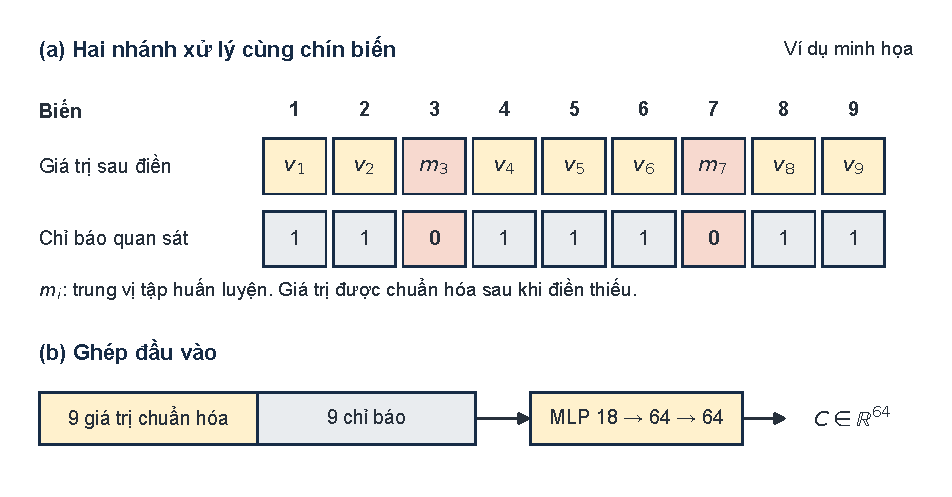
\includegraphics[width=\textwidth]{image/clinical-18-inputs.pdf}
\caption{Quy trình mở rộng chín biến lâm sàng thành 18 chiều đầu vào}
\label{fig:clinical-18}
\end{figure}

\section{Các mô hình tham chiếu}
\label{sec:architecture-evolution}
Các mô hình tham chiếu giúp trả lời hai câu hỏi: thông tin theo thời gian đóng góp thế nào, và cách kết hợp các nguồn ảnh hưởng ra sao đến dự đoán. Nhóm MRI gồm mô hình dùng ảnh cuối, mô hình dùng chuỗi MRI với trạng thái cuối của T-LSTM, và mô hình dùng T-LSTM kết hợp attention để tổng hợp cả ba trạng thái. Nhóm hợp nhất dùng cùng ba nguồn MRI, radiomics và lâm sàng, lần lượt kết hợp bằng ghép nối, tích ngoài và CP.

Một đối chứng riêng được xây dựng theo quy trình CNN--PCA--T-LSTM của Aghajanian và cộng sự \cite{aghajanian2025longitudinal}. CNN TensorFlow nhận MRI kích thước $128^3$ và xuất vectơ 512 chiều trước Dropout và lớp đầu ra. PCA được học từ tập huấn luyện với ngưỡng giữ ít nhất 99\% phương sai, không chuẩn hóa thang đo hoặc làm trắng. Chuỗi đặc trưng sau PCA được đưa vào T-LSTM có trạng thái ẩn 64 chiều.

Với các mã khởi tạo 20260727, 20260728 và 20260729, số thành phần PCA tương ứng là 38, 69 và 2. Ở lần chạy thứ ba, hai thành phần đầu đã giữ 99.47\% phương sai của 753 biểu diễn huấn luyện, nên đáp ứng ngưỡng 99\%. Phương sai tập trung rất mạnh vào hai hướng ở lần khởi tạo thứ ba, cho thấy số chiều hiệu dụng của biểu diễn CNN nhạy với khởi tạo. Mục~\ref{sec:paper-adaptation-results} đối chiếu số chiều này với C-index của từng lần khởi tạo. Bảng~\ref{tab:reference-methods} tóm tắt dữ liệu và vai trò của phương pháp gốc, bản tái lập có điều chỉnh và mô hình chính.

\begin{table}[H]
\centering\small
\caption[Phân biệt công trình gốc, bản tái lập có điều chỉnh và phương pháp chính]{Dữ liệu, cấu hình và vai trò của ba phương pháp.}
\label{tab:reference-methods}
\begin{tabularx}{\textwidth}{@{}L{3.2cm}Y Y@{}}
\toprule
\textbf{Phương pháp} & \textbf{Dữ liệu và tiền xử lý} & \textbf{Mô hình và vai trò} \\
\midrule
Aghajanian gốc \cite{aghajanian2025longitudinal} & 228 người có MCI; SPM12, mô não và radiomics chất xám & CNN--PCA--T-LSTM; huấn luyện hai bước; nguồn tham chiếu \\
Bản tái lập có điều chỉnh & 359 người; ảnh MRI đã cố định được đổi kích thước cho CNN & CNN/PCA theo lần khởi tạo; T-LSTM 64; mô hình đối chứng \\
RC-Free Pairwise & 359 người; MRI $144^3$, radiomics toàn não, lâm sàng và chỉ báo có dữ liệu & MedicalNet; CP MR/MC; phần dư có cổng; T-LSTM 128; kiến trúc chính \\
\bottomrule
\end{tabularx}
\end{table}

Về triển khai, mô hình chính dùng PyTorch và MONAI; scikit-learn thực hiện các biến đổi dữ liệu bảng \cite{paszke2019pytorch,cardoso2022monai,pedregosa2011sklearn}. Bản CNN--PCA--T-LSTM có bộ tối ưu, cỡ lô và cách tính hàm mất mát Cox khác nhóm mô hình tương tác theo cặp. C-index được tính thống nhất để đối chiếu hiệu năng tổng thể của các quy trình.

\section{Mô hình đối chứng ghép nối đặc trưng}
Đối chứng ghép nối được xây dựng để khảo sát đóng góp của tương tác theo cặp trong điều kiện giữ nguyên cả ba nguồn dữ liệu đầu vào. Tại mỗi lần khám, tôi ghép vectơ MRI $M_t$ có 128 chiều, vectơ radiomics $R_t$ có 64 chiều và vectơ lâm sàng $C_t$ có 64 chiều theo đúng thứ tự này. Khối MLP nhận vectơ chung 256 chiều và ánh xạ thành biểu diễn 128 chiều cho khối thời gian. Phép ghép nối tại lần khám $t$ có dạng
\begin{equation}
 F_t=\operatorname{MLP}_{\rm out}(M_t\concat R_t\concat C_t),\qquad
 M_t\concat R_t\concat C_t\in\mathbb R^{256},\quad F_t\in\mathbb R^{128}.\label{eq:concat}
\end{equation}
Khối đầu ra $\operatorname{MLP}_{\rm out}$ gồm lớp tuyến tính $256\to128$, GELU, Dropout 0.20 và LayerNorm. Chuỗi ba $F_t$ đi qua khối thời gian và khối dự báo Cox. Các lớp sau ghép nối học quan hệ giữa các nguồn từ vectơ chung này.


\begin{figure}[H]
\centering
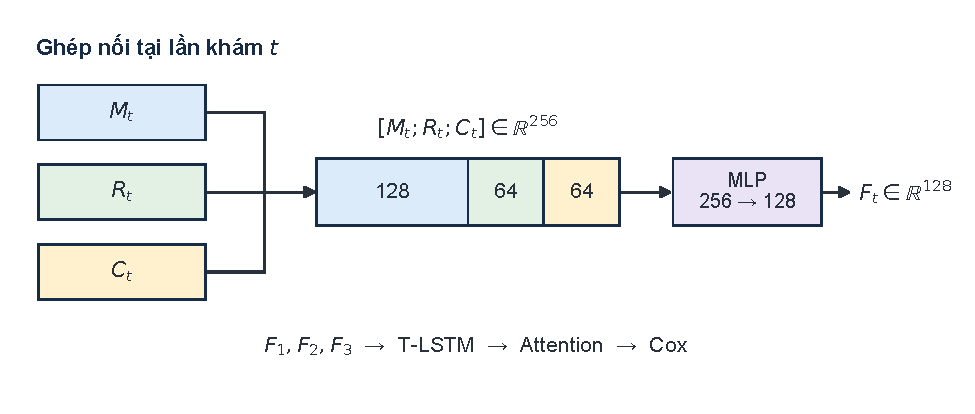
\includegraphics[width=\textwidth]{image/concat-baseline.pdf}
\caption[Mô hình đối chứng ghép nối]{Luồng tính của mô hình đối chứng ghép nối.}
\label{fig:concat-baseline}
\end{figure}
Mô hình theo cặp bổ sung một khối riêng để biểu diễn các tích chéo trước bước ghép nối. Khi so sánh hai cách hợp nhất, tôi giữ nguyên các phần chung và dùng cùng trọng số ban đầu cho các phần này. Mục~\ref{sec:matched-fusion} trình bày kết quả đối chiếu này.

\Needspace{9\baselineskip}
\section{Hợp nhất động qua tương tác theo cặp}
\label{sec:pair-fusion}
Từ cùng ba biểu diễn đầu vào như đối chứng ghép nối, mô hình đầy đủ kết hợp từng cặp tại mỗi lần khám để tạo ba tương tác MR, MC và RC. Trước khi tính tương tác, ba phép chiếu tuyến tính không có hệ số chệch giảm $M$ từ 128 xuống 32 chiều, $R$ từ 64 xuống 32 chiều và $C$ từ 64 xuống 16 chiều:
\begin{equation}
 \widetilde M\in\mathbb R^{32},\qquad
 \widetilde R\in\mathbb R^{32},\qquad
 \widetilde C\in\mathbb R^{16}.\label{eq:input-projection}
\end{equation}

\begin{figure}[H]
\centering
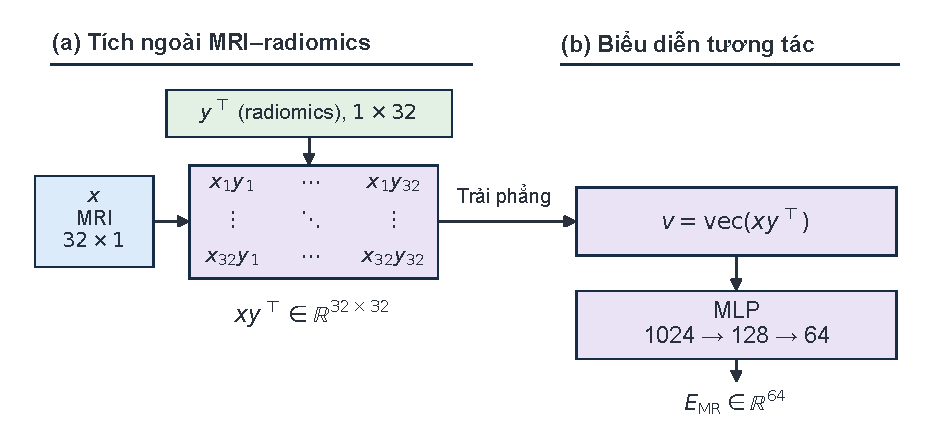
\includegraphics[width=\textwidth]{image/mr-outer-product.pdf}
\caption{Phép tích ngoài đầy đủ và khối MLP tương tác}
\label{fig:mr-outer-product}
\end{figure}

Với mỗi cặp tương tác $k\in\{\mathrm{MR},\mathrm{MC},\mathrm{RC}\}$, tôi ký hiệu hai vectơ đầu vào là $x\in\mathbb R^{d_x\times1}$ và $y\in\mathbb R^{d_y\times1}$, tương ứng với hai biểu diễn đã giảm chiều lấy từ $(\widetilde M,\widetilde R,\widetilde C)$. Tích ngoài $xy^\top\in\mathbb R^{d_x\times d_y}$ tạo ra ma trận chứa tích của từng tọa độ của $x$ với từng tọa độ của $y$, sau đó mô hình trải phẳng ma trận thành vectơ $v=\operatorname{vec}(xy^\top)$ để đưa vào MLP. Do số chiều đầu vào khác nhau giữa các cặp, MR tạo ra $32\times32=1024$ giá trị tương tác, trong khi MC và RC mỗi cặp tạo ra $32\times16=512$ giá trị.

MLP của mỗi cặp ánh xạ vectơ vừa trải phẳng thành biểu diễn tương tác: MR dùng $1024\to128\to64$, MC dùng $512\to128\to64$, RC dùng $512\to64\to32$. Giữa hai lớp tuyến tính có GELU và Dropout 0.10; LayerNorm đặt cuối mỗi khối.

Xét cặp MRI và radiomics (MR) của một người tại một lần khám. Sau khi xử lý cặp này, MLP cho một vectơ 64 chiều biểu diễn thông tin tương tác giữa hai nguồn. Mô hình dùng vectơ đó để bổ sung thông tin cho cả biểu diễn MRI $M$ và biểu diễn radiomics $R$. Vì phép cộng được thực hiện theo từng tọa độ, phần bổ sung phải có cùng số chiều với biểu diễn nhận nó.

Hình~\ref{fig:pair-update-routes} minh họa hai nhánh đi ra từ MR. Ở nhánh dẫn đến MRI, một lớp tuyến tính biến vectơ tương tác 64 chiều thành vectơ 128 chiều để có thể cộng vào $M$. Ở nhánh dẫn đến radiomics, một lớp tuyến tính khác ánh xạ từ 64 chiều sang 64 chiều. Dù số chiều đã khớp với $R$, lớp này vẫn học cách kết hợp các tọa độ của vectơ tương tác cho riêng nguồn radiomics. Sau phép chiếu, mỗi nhánh chuẩn hóa vectơ bằng LayerNorm riêng. Cổng của nhánh điều tiết mức đóng góp tại lần khám đang xét. Mô hình nhân vectơ đã chuẩn hóa với giá trị cổng và hệ số của nhánh trước khi cộng vào biểu diễn gốc.

\begin{figure}[H]
\centering
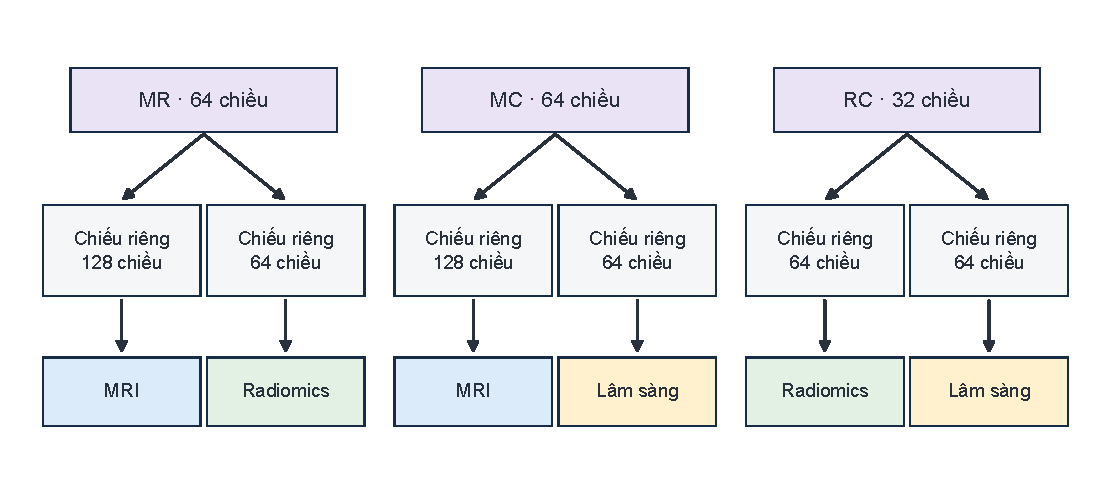
\includegraphics[width=\linewidth]{image/pair-update-routes.pdf}
\caption{Sơ đồ sáu nhánh cập nhật biểu diễn từ ba cặp tương tác}
\label{fig:pair-update-routes}
\end{figure}

Đọc sơ đồ theo nguồn nhận cho thấy MRI nhận thông tin từ MR và MC, radiomics nhận từ MR và RC, còn dữ liệu lâm sàng nhận từ MC và RC. Mỗi nguồn giữ vectơ gốc và cộng các phần bổ sung dành cho mình. Cả sáu nhánh đều sử dụng dữ liệu của cùng một người ở cùng một lần khám. Khi bỏ cặp RC, hai nhánh từ RC đến radiomics và lâm sàng cũng được bỏ. Trong RC-Free, radiomics vẫn nhận thông tin từ MR và dữ liệu lâm sàng vẫn nhận thông tin từ MC, nên cả ba nguồn tiếp tục tham gia vào biểu diễn hợp nhất.

\section{Tham số hóa tương tác theo cặp bằng CP}
\label{sec:cp-method}

Mặc dù phép hợp nhất tương tác song tuyến đầy đủ (Full Outer-Product) ở Mục~\ref{sec:pair-fusion} có khả năng bắt cặp tường minh các đặc trưng giữa hai phương thức, rào cản lớn nhất của nó nằm ở chi phí tính toán và số lượng tham số khổng lồ. Một lớp song tuyến đầy đủ đòi hỏi phải học một tensor trọng số ba chiều $\mathcal W\in\mathbb R^{d_h\times d_x\times d_y}$. Khi số chiều đặc trưng hoặc số kênh ẩn tăng lên, số lượng tham số này bùng nổ rất nhanh, không chỉ gây áp lực lớn lên bộ nhớ tính toán mà còn làm tăng nghiêm trọng nguy cơ quá khớp (overfitting) trên các bộ dữ liệu y tế vốn có cỡ mẫu hạn chế như ADNI.

Để giải quyết mâu thuẫn giữa năng lực biểu diễn tương tác và độ phức tạp tham số, tôi áp dụng kỹ thuật phân rã tensor CANDECOMP/PARAFAC (CP) \cite{kolda2009tensor,liu2018lowrank}. Nguyên lý cốt lõi của phân rã CP là xấp xỉ tensor trọng số ba chiều phức tạp thành tổng của $Q$ tích ngoài giữa các vectơ một chiều, trong đó $Q \ll \min(d_x d_y, d_h)$ là hạng phân rã (rank). Nhờ cấu trúc hạng thấp này, thay vì phải thực hiện tích ngoài tường minh trong không gian gốc, hai vectơ đặc trưng đầu vào trước hết được chiếu tuyến tính về một không gian tiềm ẩn thấp chiều ($Q$ chiều), sau đó nhân từng phần tử (Hadamard product) để tạo tương tác, rồi mới chiếu tiếp sang không gian ẩn $d_h$. Hình~\ref{fig:cp-block} minh họa trực quan luồng tính toán này cho cặp MR với hạng $Q=8$.

\begin{figure}[H]
\centering
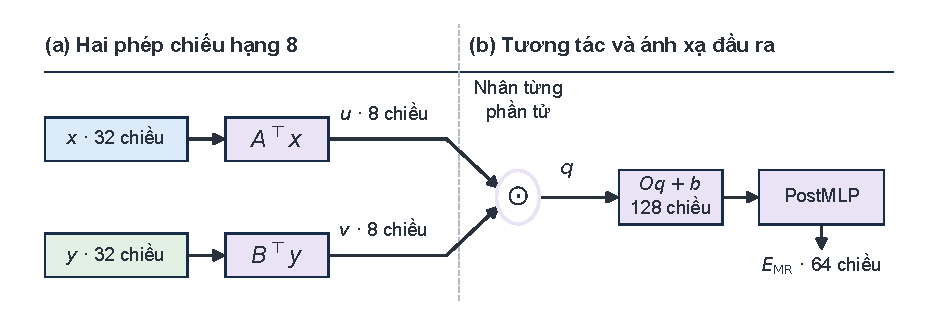
\includegraphics[width=\textwidth]{image/outer-vs-cp.pdf}
\caption{Luồng tính toán của khối tương tác CP hạng thấp}
\label{fig:cp-block}
\end{figure}
Với lớp đầy đủ, chiều ẩn thứ $s$ được tính bằng
\begin{equation}
 h_s=\sum_{i=1}^{d_x}\sum_{j=1}^{d_y}\mathcal W_{sij}x_i y_j+b_s,
 \qquad \mathcal W\in\mathbb R^{d_h\times d_x\times d_y}.
\end{equation}
Thay vì phải lưu trữ và học trực tiếp toàn bộ khối trọng số khổng lồ trên, CP tham số hóa \emph{tensor trọng số của ánh xạ song tuyến} thông qua các ma trận nhân tử hạng thấp \cite{kolda2009tensor,liu2018lowrank}:
\begin{equation}
 \mathcal W_{sij}\approx\sum_{q=1}^{Q}O_{sq}A_{iq}B_{jq}.
 \label{eq:cp-weight}
\end{equation}
Trong cách biểu diễn phân rã này, mạng chỉ cần học ba ma trận nhân tử $A\in\mathbb R^{d_x\times Q}$, $B\in\mathbb R^{d_y\times Q}$ và $O\in\mathbb R^{d_h\times Q}$. Quá trình tính toán thuận diễn ra hết sức tự nhiên và hiệu quả: hai vectơ đầu vào $x$ và $y$ được chiếu độc lập về không gian $Q$ chiều thông qua $A$ và $B$, tạo thành hai vectơ tọa độ $u$ và $v$; tiếp đó, phép nhân từng phần tử giữa $u$ và $v$ nắm bắt tương tác chéo giữa hai nguồn dữ liệu; cuối cùng, ma trận $O$ chiếu kết quả tương tác này lên không gian ẩn $d_h$:
\begin{align}
 u&=A^\top x,\qquad v=B^\top y,\qquad q=u\odot v,\label{eq:cp-lowrank}\\
 h&=Oq+b,\qquad E_k=\operatorname{PostMLP}_k(h),
 \label{eq:cpblock}
\end{align}
với $E_k$ là biểu diễn tương tác đầu ra của cặp $k\in\{\mathrm{MR},\mathrm{MC},\mathrm{RC}\}$. Cần lưu ý rằng các ma trận chiếu $A$ và $B$ không sử dụng hệ số chệch để bảo toàn tính đối xứng của phép nhân từng phần tử; hệ số chệch $b$ của lớp đầu được tích hợp trực tiếp vào phép chiếu đầu ra $Oq+b$. Khối mạng perceptron đa tầng phía sau ($\operatorname{PostMLP}_k$) vẫn giữ nguyên cấu trúc chuẩn hóa và phi tuyến gồm hàm kích hoạt GELU, Dropout 0.10, lớp tuyến tính $d_h\to d_o$ và chuẩn hóa LayerNorm. Nhờ vậy, mô hình đối chứng CP chỉ thay đổi duy nhất phép biến đổi tương tác đầu tiên, trong khi bảo lưu toàn bộ kích thước đầu ra, MLP phía sau, bộ mã hóa, các nhánh truyền phần dư, cổng điều tiết, hệ số điều chỉnh và khối thời gian. Cách bố trí này giúp cô lập hoàn toàn biến số nghiên cứu, bảo đảm rằng bất kỳ sự khác biệt nào về hiệu năng đều phản ánh chính xác hiệu quả của việc tham số hóa hạng thấp.



\begin{table}[H]
\centering
\caption{Cấu hình CP theo cặp tương tác}
\label{tab:cpconfig}
\begin{tabular}{lccccc}
\toprule
Cặp & $(d_x,d_y)$ & Hạng $Q$ & Chiều ẩn $d_h$ & Đầu ra $d_o$ & RC-Free \\
\midrule
MR & $(32,32)$ & 8 & 128 & 64 & Giữ \\
MC & $(32,16)$ & 8 & 128 & 64 & Giữ \\
RC & $(32,16)$ & 4 & 64 & 32 & Loại \\
\bottomrule
\end{tabular}
\end{table}

Bảng~\ref{tab:cpconfig} trình bày chi tiết cấu hình hạng CP và kích thước các lớp cho từng cặp tương tác. Việc ấn định hạng $Q=8$ cho hai cặp MR và MC cùng $Q=4$ cho cặp RC phản ánh sự cân đối có chủ đích giữa năng lực biểu diễn và kích thước đặc trưng của từng phương thức (cặp RC có số chiều đầu vào nhỏ hơn nên chỉ cần hạng thấp hơn).

Hiệu quả giảm độ phức tạp của phân rã CP có thể được định lượng rõ ràng qua sự khác biệt giữa hai công thức tham số: một lớp song tuyến đầy đủ đòi hỏi $d_h d_x d_y + d_h$ tham số (với độ phức tạp tăng theo tích $d_x d_y$), trong khi cách tham số hóa CP chỉ tiêu tốn $Q(d_x + d_y + d_h) + d_h$ tham số (với độ phức tạp chỉ tăng tuyến tính theo tổng $d_x + d_y$). Đây chính là nền tảng lý thuyết giải thích vì sao CP có thể \textbf{cắt giảm hơn 98\%} số lượng trọng số ở các lớp tương tác đầu tiên. Dẫu vậy, xét trên quy mô toàn mạng, bộ mã hóa hình ảnh 3D ResNet-18 vẫn chiếm phần lớn số tham số; do đó, vai trò cốt lõi của CP không chỉ là thu nhỏ mô hình tổng thể, mà quan trọng hơn là đóng vai trò như một cơ chế điều chuẩn (regularization) hiệu quả, ngăn chặn hiện tượng quá khớp ở chính các tầng hợp nhất đa phương thức.

\section{Truyền phần dư qua cổng điều tiết động}
\label{sec:gated-routing}

Sau khi đã trích xuất được đặc trưng tương tác từ các khối CP, bài toán kiến trúc cốt lõi tiếp theo là: \emph{Làm thế nào để truyền tải và tích hợp thông tin tương tác này vào biểu diễn của từng phương thức mà không làm suy hao hoặc sai lệch tín hiệu gốc?}

Trong mô hình đối chứng ghép nối thông thường, các đặc trưng được gộp cứng nhắc lại với nhau trước khi đưa vào mô hình thời gian. Cách tiếp cận này tiềm ẩn nhiều rủi ro trong bài toán y sinh: sự tương tác giữa các phương thức không phải lúc nào cũng mang lại giá trị gia tăng đồng đều ở mọi bệnh nhân hay mọi thời điểm thăm khám. Ở một số ca bệnh hoặc lần khám có độ nhiễu cao (chẳng hạn chất lượng ảnh MRI kém hoặc kết quả đo lâm sàng dao động), việc ép buộc mô hình tiếp nhận toàn bộ tín hiệu tương tác có thể làm xáo trộn các đặc trưng bệnh học vốn có của từng nguồn đơn lẻ.

Để khắc phục nhược điểm này, tôi đề xuất cơ chế \emph{kết nối phần dư qua cổng điều tiết động} (gated residual routing), kế thừa và phát triển từ các nguyên lý điều tiết phần dư trong học sâu đa phương thức \cite{ryumina2026residual,liu2026motion}. Triết lý của cơ chế này là bảo toàn nguyên vẹn ``đường truyền gốc'' (identity path) của từng phương thức, đồng thời xem thông tin tương tác như một lượng bổ chính phần dư có điều kiện. Nhờ đó, ngay cả khi tín hiệu tương tác bị nhiễu hoặc cổng điều tiết khép lại, mô hình vẫn duy trì được nguồn thông tin độc lập và tin cậy từ biểu diễn ban đầu.

Cơ chế điều tiết này được hiện thực hóa qua ba tầng xử lý chặt chẽ:
\begin{enumerate}
\item \emph{Phép chiếu tương thích theo phương thức đích}: Mỗi cặp tương tác $k$ (như MR hay MC) tạo ra một biểu diễn tương tác chung $E_k$. Tuy nhiên, do các phương thức đích $d$ có kích thước không gian đặc trưng khác nhau, đặc trưng $E_k$ trước tiên được chiếu về không gian của phương thức đích thông qua một ánh xạ tuyến tính và chuẩn hóa qua LayerNorm:
\begin{equation}
 \widehat E_{k\to d}=\LN_{k\to d}(W_{k\to d}E_k+b_{k\to d}).\label{eq:target-projection}
\end{equation}
Ánh xạ này sử dụng hệ số chệch để tăng tính linh hoạt khi dịch chuyển hệ tọa độ đặc trưng, trong khi bước giảm chiều trước CP hoàn toàn không dùng hệ số chệch. Cả hai bước đều không sử dụng hàm kích hoạt phi tuyến nhằm bảo toàn tuyến tính của tín hiệu trước khi vào cổng.

\item \emph{Cổng điều tiết động theo từng bệnh nhân}: Cổng $g_{k\to d}$ hoạt động như một chiếc ``van thông minh'', tiếp nhận đồng thời cả biểu diễn gốc đã chuẩn hóa của phương thức đích lẫn đặc trưng tương tác đã chiếu để đánh giá xem: với \emph{cá thể cụ thể này tại lần khám cụ thể này}, thông tin tương tác có thực sự hữu ích hay không:
\begin{equation}
 g_{k\to d}=\sigma\!\left(
 w_{k\to d}^{\top}\operatorname{GELU}\!\left[
 V_{k\to d}\bigl(\LN_d^{\rm gate}(U_d)\concat\widehat E_{k\to d}\bigr)
 +a_{k\to d}\right]+c_{k\to d}\right).
 \label{eq:dynamic-gate}
\end{equation}
Mạng MLP của mỗi cổng gồm một lớp ẩn 32 chiều với kích hoạt GELU và tạo ra một giá trị vô hướng trong khoảng $(0,1)$ thông qua hàm sigmoid độc lập. Việc sử dụng sigmoid riêng cho từng cổng (thay vì softmax trên tất cả các nhánh) mang ý nghĩa then chốt: các nhánh tương tác có thể cùng mở rộng nếu tất cả đều hữu ích, hoặc cùng khép lại nếu dữ liệu bị nhiễu, mà không bị ràng buộc phải chia sẻ một tổng trọng số cố định. Trọng số của cổng được khởi tạo theo phân phối Xavier~\cite{glorot2010understanding} với hệ số chệch ban đầu bằng không.

\item \emph{Hệ số tỉ lệ toàn cục học được}: Bên cạnh chiếc van động $g_{k\to d}$ điều chỉnh theo từng mẫu, mỗi nhánh còn được trang bị một hệ số vô hướng $\lambda_{k\to d}$ dùng chung cho toàn bộ tập dữ liệu và mọi mốc thời gian. Hệ số này được khởi tạo tại $\lambda=0.1$ và \emph{hoàn toàn không bị ràng buộc về dấu}. Nếu cổng $g$ quyết định độ mở tức thời theo ngữ cảnh của từng bệnh nhân, thì $\lambda$ đóng vai trò như một ``chiết áp nền'' học được trong quá trình tối ưu, xác định cường độ đóng góp tổng thể và chiều hướng tác động (tương hỗ tích cực hay triệt tiêu lẫn nhau) của toàn bộ nhánh truyền.
\end{enumerate}

\begin{figure}[H]
\centering
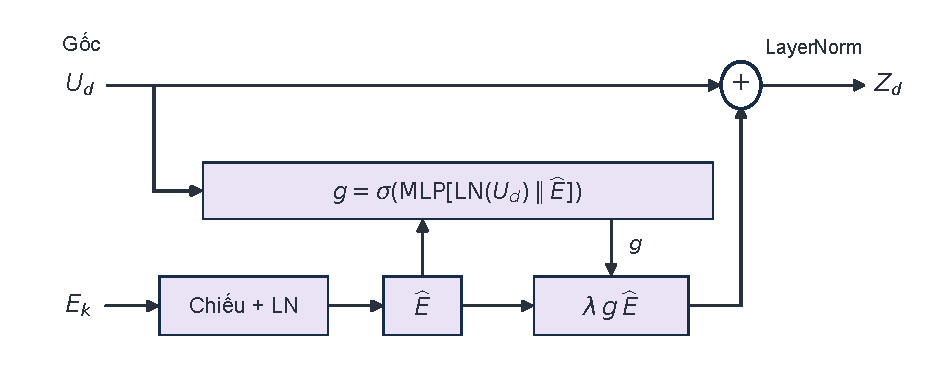
\includegraphics[width=\textwidth]{image/gated-residual-route.pdf}
\caption{Cấu trúc một nhánh phần dư có cổng điều tiết động}
\label{fig:route}
\end{figure}

Tổng hợp lại, biểu diễn của phương thức đích $d$ sau khi nhận các luồng bổ chính tương tác được xác định bởi:
\begin{equation}
 Z_d=\LN_d^{\rm out}\left(
 U_d+\sum_{k\in\mathcal P(d)}\lambda_{k\to d}\,g_{k\to d}\,\widehat E_{k\to d}
 \right),
 \label{eq:ours-residual}
\end{equation}
trong đó $\mathcal P(d)$ là tập hợp các cặp tương tác còn hoạt động hướng tới phương thức đích $d$. Cần nhấn mạnh rằng ba phép chuẩn hóa LayerNorm xuất hiện trong quy trình — tại phép chiếu đích ($\LN_{k\to d}$), tại đầu vào cổng ($\LN_d^{\rm gate}$), và sau tổng phần dư ($\LN_d^{\rm out}$) — là ba tầng chuẩn hóa hoàn toàn độc lập với các tham số riêng biệt \cite{ba2016layernorm}. Sự phân tách này ngăn ngừa hiện tượng dịch chuyển phân phối và kiểm soát chặt chẽ biên độ tín hiệu qua các tầng, giúp việc huấn luyện mô hình luôn duy trì được độ ổn định số học cao. Mức đóng góp thực tế của thông tin tương tác vì vậy phụ thuộc đồng thời vào độ mở của cổng, hệ số $\lambda$ và độ lớn của đặc trưng: khi cổng khép gần về 0, nhánh tương tác gần như bị triệt tiêu để bảo vệ biểu diễn gốc; ngược lại, khi cổng mở gần về 1, tín hiệu tương tác sau khi được điều chỉnh biên độ sẽ hòa nhập tối đa vào dòng chảy đặc trưng của phương thức đích.

\section{Cấu trúc RC-Free}
\label{sec:rcfree-method}

Trong mô hình tích ngoài CP đầy đủ (Full CP), ta xem xét toàn bộ ba cặp tương tác có thể có giữa ba phương thức: MR, MC và RC, dẫn đến việc phải duy trì tới sáu nhánh truyền phần dư có cổng. Tuy nhiên, một câu hỏi kiến trúc mang tính bản chất nảy sinh: \emph{Liệu có nhất thiết phải thiết lập tương tác trực tiếp giữa tất cả các cặp, hay một cấu trúc tinh giản hơn vẫn có thể đạt hiệu quả tương đương, thậm chí vượt trội hơn?}

Xét về bản chất y sinh và hình ảnh học của các nguồn dữ liệu trong bài toán dự báo Alzheimer: ảnh MRI là dữ liệu hình ảnh cấu trúc ba chiều nguyên bản, phản ánh hình thái và mức độ teo thoái hóa của toàn bộ não bộ; các đặc trưng Radiomics là những chỉ số kết cấu định lượng được trích xuất từ chính các vùng não trên ảnh MRI đó; trong khi dữ liệu lâm sàng (Clinical) phản ánh tình trạng nhận thức và hoạt động chức năng toàn diện của người bệnh. Rõ ràng, hình ảnh MRI đóng vai trò như một ``mỏ neo'' thông tin trung tâm, có mối liên hệ mật thiết cả với đặc trưng vi mô của mô não (thông qua Radiomics) lẫn biểu hiện bệnh học vĩ mô (thông qua Clinical). Ngược lại, mối tương tác trực tiếp giữa Radiomics và Clinical (cặp RC) khi không có sự tham chiếu của hình ảnh MRI gốc có thể trở nên dư thừa, hoặc thậm chí tạo ra các tương quan giả (spurious correlations) do nhiễu đo lường trên các thang điểm nhận thức.

Từ nhận định sâu sắc trên, tôi đề xuất kiến trúc \textbf{RC-Free} (loại bỏ cặp tương tác Radiomics--Clinical). Trong thiết kế này, khối tương tác trực tiếp RC được lược bỏ hoàn toàn, đặt biểu diễn hình ảnh MRI làm ``trung tâm kết nối'' cho hai tương tác cốt lõi: MRI--Radiomics (MR) và MRI--Clinical (MC).

Hình~\ref{fig:rcfree-update} trực quan hóa cơ chế truyền thông tin tinh gọn của RC-Free tại một lần khám. Nhìn vào sơ đồ, luồng dữ liệu diễn ra như sau:
\begin{itemize}
\item Cả ba phương thức đầu vào vẫn được duy trì đầy đủ, bảo đảm không làm mất bất kỳ nguồn thông tin nào.
\item Số nhánh truyền phần dư có cổng được tinh giản từ sáu xuống còn bốn nhánh: hình ảnh MRI nhận thông tin bổ chính từ cả hai tương tác MR và MC; đặc trưng Radiomics nhận bổ chính từ MR; và dữ liệu lâm sàng nhận bổ chính từ MC.
\item Radiomics và dữ liệu lâm sàng tuy không tương tác trực tiếp với nhau, nhưng vẫn được liên kết gián tiếp thông qua trung tâm MRI trước khi các biểu diễn được ghép nối thành một vectơ thống nhất.
\end{itemize}

\begin{figure}[H]
\centering
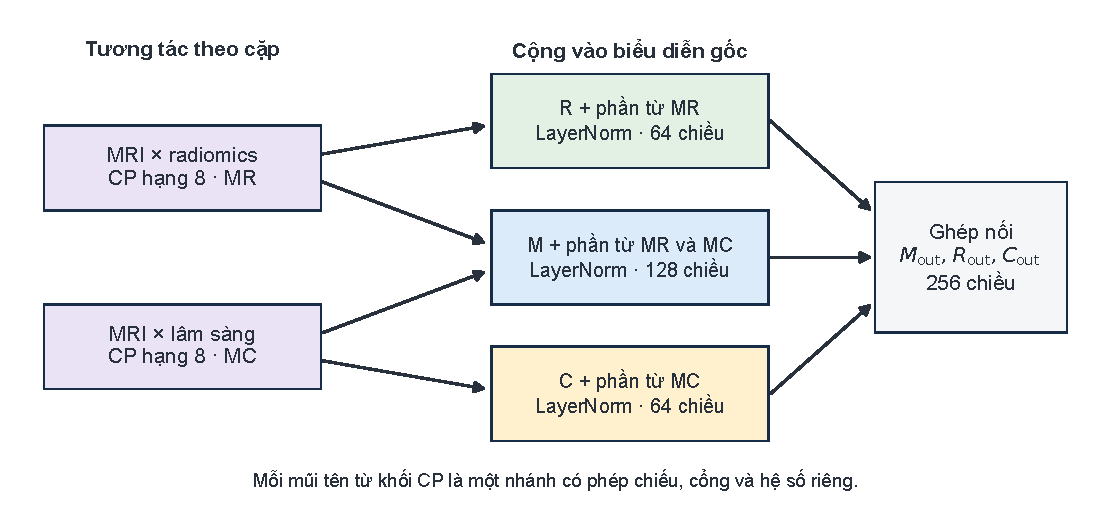
\includegraphics[width=\linewidth]{image/rcfree-update.pdf}
\caption{Bốn nhánh cập nhật đặc trưng trong mô hình RC-Free}
\label{fig:rcfree-update}
\end{figure}

Đặt $D_{k\to d}=\lambda_{k\to d}g_{k\to d}\widehat E_{k\to d}$ là lượng bổ chính tương tác từ cặp $k$ sang phương thức $d$, các phương trình cập nhật đặc trưng trong RC-Free được xác định như sau:
\begin{align}
 M_{\rm out}&=\LN_M^{\rm out}(M+D_{(\mathrm{MR}\to M)}+D_{(\mathrm{MC}\to M)}),\label{eq:rcfree-first}\\
 R_{\rm out}&=\LN_R^{\rm out}(R+D_{(\mathrm{MR}\to R)}),\\
 C_{\rm out}&=\LN_C^{\rm out}(C+D_{(\mathrm{MC}\to C)}).
 \label{eq:rcfree-residual}
\end{align}

Cụ thể, hai khối CP cho MR và MC đều được ấn định hạng $Q=8$. Bốn nhánh truyền tương ứng được kiểm soát bởi bốn phép chiếu theo đích, bốn cổng động độc lập và bốn hệ số điều chỉnh $\lambda$ học được. Sau các phép cộng phần dư và chuẩn hóa LayerNorm, các biểu diễn đầu ra $M_{\rm out}, R_{\rm out}, C_{\rm out}$ lần lượt có kích thước 128, 64 và 64 chiều. Ba vectơ này sau đó được ghép nối liên tiếp thành vectơ đặc trưng đa phương thức $F_t \in \mathbb R^{256}$ tại mỗi lần khám $t$, sẵn sàng làm đầu vào cho khối mô hình hóa chuỗi thời gian tiếp theo. Nhờ việc giữ nguyên kích thước sau ghép nối này, việc chuyển từ Full CP sang RC-Free không làm thay đổi cấu trúc của bất kỳ tầng tính toán nào phía sau, tạo điều kiện thuận lợi để đối chiếu hiệu năng một cách công bằng.

\section{Mô hình thời gian và attention}
\label{sec:temporal-method}

Sau khi đã thu được các vectơ đặc trưng đa phương thức $F_t$ tại từng thời điểm thăm khám, nhiệm vụ tiếp theo là mô hình hóa tiến trình suy giảm bệnh lý theo chiều thời gian. Dự báo tiến triển bệnh Alzheimer đòi hỏi phải khai thác dữ liệu quan sát dọc (longitudinal data). Tuy nhiên, bài toán y sinh thực tế đặt ra hai thách thức lớn mà các kiến trúc học sâu tuần tự thông thường không thể xử lý thỏa đáng:
\begin{enumerate}
\item \emph{Khoảng cách thời gian không đồng đều giữa các lần khám}: Khác với các chuỗi thời gian lý thuyết có chu kỳ đo lường cố định, người bệnh trong các nghiên cứu lâm sàng như ADNI tái khám theo những khoảng thời gian biến thiên thực tế (có khi 6 tháng, có khi 1 năm hoặc lâu hơn). Một mạng LSTM tiêu chuẩn vốn giả định các bước thời gian cách đều nhau, do đó sẽ đánh đồng khoảng cách vài tháng với khoảng cách hàng năm, bỏ qua quy luật bệnh học hiển nhiên: khoảng cách giữa hai lần chụp càng dài thì các biến động tức thời từ lần khám trước càng bị suy giảm và khó dự đoán hơn.

\item \emph{Độ quan trọng không đồng đều giữa các mốc thăm khám}: Các dấu hiệu thoái hóa thần kinh then chốt (như teo hồi hải mã hay tụt dốc điểm nhận thức) không diễn ra dàn trải mà thường bộc lộ rõ nét tại một số thời điểm chuyển giai đoạn nhất định. Do đó, việc chỉ lấy trạng thái ẩn ở bước cuối cùng $h_T$ có thể làm mất mát các tín hiệu cảnh báo sớm ở giai đoạn đầu, trong khi lấy trung bình cộng lại làm loãng các thông tin quan trọng.
\end{enumerate}

Để giải quyết trọn vẹn thách thức thứ nhất, tôi tích hợp mạng Time-Aware LSTM (T-LSTM) \cite{baytas2017patient,aghajanian2025longitudinal}. Nguyên lý cốt lõi của T-LSTM là sử dụng trực tiếp khoảng thời gian thực tế trôi qua giữa hai lần khám để điều chỉnh trạng thái bộ nhớ của mạng. Cụ thể, khoảng thời gian tại lần khám đầu tiên được quy ước bằng không. Tại các lần khám tiếp theo $t \geq 2$, khoảng cách thực tế giữa hai lần chụp liên tiếp $s_t$ và $s_{t-1}$ (tính theo ngày) được quy đổi sang đơn vị năm: $\Delta t_t = (s_t - s_{t-1}) / 365.25$. T-LSTM sử dụng trực tiếp khoảng thời gian này để điều chỉnh trạng thái bộ nhớ mà không cần bổ sung một biểu diễn thời gian được học riêng.

Từ bộ nhớ trước đó $c_{t-1}$, mô hình tách thành phần ngắn hạn $c_{t-1}^{S}$ (chứa các biến động tức thời) và phần còn lại $c_{t-1}^{L}$ (chứa các đặc trưng bệnh lý bền vững), rồi điều chỉnh theo hệ số suy giảm phi tuyến $\gamma_t$:
\begin{align}
 c_{t-1}^{S}&=\tanh(W_Sc_{t-1}+b_S),\qquad
 c_{t-1}^{L}=c_{t-1}-c_{t-1}^{S},\label{eq:tlstm-first}\\
 \gamma_t&=\frac{1}{\log(e+\Delta t_t)},\qquad
 c_{t-1}^{*}=c_{t-1}^{L}+\gamma_t c_{t-1}^{S}.
 \label{eq:tlstm-memory}
\end{align}
Khi $\Delta t_t$ càng lớn, $\gamma_t$ càng giảm, phản ánh chính xác hiện tượng thông tin ngắn hạn từ quá khứ xa bị phai mờ tự nhiên. Bộ nhớ hiệu chỉnh $c_{t-1}^{*}$ này sau đó được đưa vào các cổng cập nhật của LSTM:
\begin{equation}
 c_t=f_t\odot c_{t-1}^{*}+i_t\odot\widetilde c_t,
 \qquad h_t=o_t\odot\tanh(c_t).\label{eq:tlstm-state}
\end{equation}
Trong đó, các cổng đầu vào $i_t$, quên $f_t$, đầu ra $o_t$ và bộ nhớ ứng viên $\widetilde c_t$ được tính từ $F_t$ và $h_{t-1}$ bằng các ánh xạ tuyến tính có hệ số chệch (dùng sigmoid cho các cổng và tanh cho bộ nhớ ứng viên). T-LSTM gồm một lớp một chiều với trạng thái ẩn 128 chiều. Nếu một lần khám được đánh dấu không hợp lệ, mô hình giữ trạng thái trước đó; trong nhóm nghiên cứu này, cả ba lần khám của mỗi người đều hợp lệ.

\begin{figure}[H]
\centering
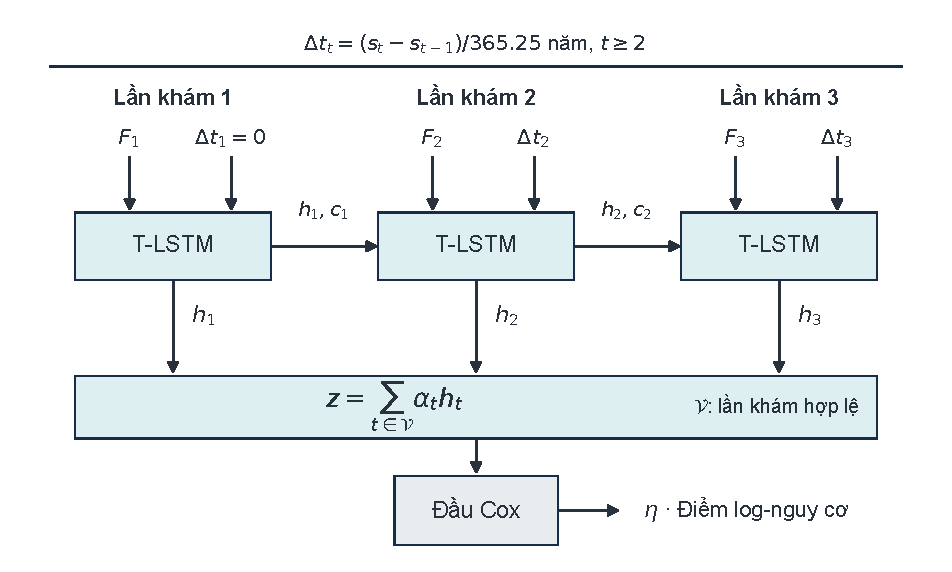
\includegraphics[width=\textwidth]{image/temporal-model.pdf}
\caption{Mô hình thời gian T-LSTM và cơ chế attention}
\label{fig:temporal}
\end{figure}

Để giải quyết thách thức thứ hai, tôi tiếp tục xây dựng một cơ chế Attention cộng theo thời gian (additive temporal attention) \cite{bahdanau2015attention} đặt phía sau T-LSTM, như được minh họa trong Hình~\ref{fig:temporal}. Cơ chế này học cách gán trọng số thích ứng cho từng lần khám:
\begin{equation}
 e_t=v_a^\top\tanh(W_a h_t+b_a),\qquad
 \alpha_t=\frac{\exp(e_t)}{\sum_{j\in\mathcal V}\exp(e_j)},\qquad
 z=\sum_{t\in\mathcal V}\alpha_t h_t.
 \label{eq:temporal-attention}
\end{equation}
Ở đây, $\mathcal V$ là tập hợp các lần khám hợp lệ. Phép chiếu $128\to64\to1$ chấm điểm từng trạng thái ẩn để xác định trọng số $\alpha_t$ của trạng thái đó trong biểu diễn tổng hợp $z\in\mathbb R^{128}$. Sự kết hợp giữa T-LSTM và Attention mang lại một cơ chế mô hình hóa thời gian toàn diện: T-LSTM đảm nhận việc tích lũy và điều tiết dòng chảy lịch sử theo khoảng cách thực tế, còn Attention đảm nhận việc chắt lọc những dấu mốc then chốt để tạo nên biểu diễn chung phục vụ cho bài toán tiên lượng sống còn.

\section{Hàm mục tiêu Cox}
\label{sec:training-method}

Từ biểu diễn chuỗi đã tổng hợp $z$, mục tiêu cuối cùng là dự đoán nguy cơ tiến triển suy giảm nhận thức trong tương lai. Bài toán này không thể giải quyết bằng các hàm mất mát phân loại nhị phân thông thường (như Cross-Entropy), bởi lẽ trong dữ liệu y tế theo dõi dọc, phần lớn người tham gia là dữ liệu kiểm duyệt phải (right-censored) — tức là đến thời điểm nghiên cứu kết thúc hoặc lần tái khám cuối cùng, họ vẫn chưa biểu hiện suy giảm nhận thức. Nếu loại bỏ những bệnh nhân này, mô hình sẽ mắc sai lệch chọn mẫu nghiêm trọng; còn nếu gắn nhãn họ là ``không bệnh'', mô hình sẽ bỏ qua khoảng thời gian họ đã duy trì tình trạng ổn định.

Để giải quyết triệt để bài toán sống còn có kiểm duyệt, tôi đưa biểu diễn $z$ qua một khối mạng perceptron đa tầng tiên lượng gồm lớp tuyến tính $128\to64$, kích hoạt GELU, Dropout 0.30 và lớp tuyến tính $64\to1$ để tính một giá trị log-nguy cơ vô hướng $\eta_i$ cho từng cá thể $i$. Điểm này được đưa trực tiếp vào mô hình nguy cơ tỷ lệ Cox \cite{cox1972regression} mà không qua bất kỳ hàm kích hoạt phi tuyến nào:
\begin{equation}
 h(\tau\mid z_i)=h_0(\tau)\exp(\eta_i),
\end{equation}
trong đó $h(\tau\mid z_i)$ là hàm nguy cơ tức thời tại thời điểm $\tau$, còn $h_0(\tau)$ là hàm nguy cơ nền chung. Theo mô hình này, tại bất kỳ thời điểm nào, người có chỉ số log-nguy cơ $\eta_i$ cao hơn sẽ có nguy cơ tức thời gặp biến cố suy giảm nhận thức lớn hơn theo cấp số mũ.

Hàm mất mát để huấn luyện mạng được xây dựng dựa trên nguyên lý đối log-hợp lý riêng phần (negative partial log-likelihood), xử lý các trường hợp trùng thời điểm biến cố theo quy tắc Breslow \cite{breslow1974covariance} và lấy trung bình trên $N_e$ biến cố quan sát được:
\begin{equation}
 \mathcal L_{\rm Cox}=-\frac{1}{N_e}\sum_k
 \left[\sum_{i\in\mathcal D_k}\eta_i
 -d_k\log\!\left(\sum_{j\in\mathcal R_k}\exp(\eta_j)\right)\right].
 \label{eq:cox-method}
\end{equation}
Ở đây, $\tau_k$ là các mốc thời gian ghi nhận biến cố phân biệt, $\mathcal D_k$ là tập hợp những người xảy ra biến cố tại $\tau_k$ với số lượng $d_k=|\mathcal D_k|$, và $\mathcal R_k=\{j:t_j\geq\tau_k\}$ là tập nguy cơ gồm tất cả những người vẫn đang được theo dõi và chưa gặp biến cố ngay trước thời điểm $\tau_k$.

Ý nghĩa cốt lõi của hàm mất mát Cox nằm ở cơ chế ``so kè thứ tự'': tại mỗi thời điểm một người gặp biến cố, mô hình phạt nặng nếu điểm nguy cơ $\eta_i$ của người đó không vượt trội so với điểm số của tất cả những người khác vẫn đang an toàn trong tập nguy cơ $\mathcal R_k$. Nhờ cơ chế này, ngay cả những người bị kiểm duyệt (không có biến cố) vẫn đóng góp tích cực vào việc huấn luyện mạng bằng cách đóng vai trò làm nhóm chứng so sánh trong tập nguy cơ cho đến tận ngày khám cuối cùng của họ.

Thuật toán~\ref{alg:rcfree-forward} tóm lược toàn bộ luồng tính toán xuôi (forward pass) của mô hình RC-Free từ lúc tiếp nhận ba nguồn dữ liệu thô tại ba lần khám cho đến khi xuất ra điểm log-nguy cơ phục vụ tối ưu hóa hàm mất mát Cox. Các bộ mã hóa và khối hợp nhất dùng chung trọng số qua ba lần khám; bốn nhánh tương tác có cổng được tính từ các biểu diễn trong cùng một lần khám.
\begin{algorithm}[H]
\caption{Luồng tính xuôi của mô hình RC-Free Pairwise Fusion}
\label{alg:rcfree-forward}
\small
\textbf{Đầu vào:} Chuỗi ba lần khám $(t=1,2,3)$ của một cá thể gồm ảnh MRI đã tiền xử lý, vectơ đặc trưng radiomics sau PCA (16 chiều), vectơ lâm sàng kèm chỉ báo quan sát (18 chiều) và khoảng cách thời gian $\Delta t_t$ (với $\Delta t_1=0$).\\
\textbf{Đầu ra:} Điểm log-nguy cơ $\eta\in\mathbb R$ của cá thể.
\begin{enumerate}[leftmargin=1.2em,label=\arabic*.,itemsep=0.2em]
\item Với mỗi lần khám $t=1,2,3$:
\begin{enumerate}[leftmargin=1.2em,label=\alph*.,itemsep=0.15em]
\item Mã hóa ba nguồn đầu vào tại lần khám $t$ thành $M_t\in\mathbb R^{128}$, $R_t\in\mathbb R^{64}$, $C_t\in\mathbb R^{64}$ theo Mục~\ref{sec:preprocessing}; chiếu tuyến tính không hệ số chệch về $\widetilde M_t\in\mathbb R^{32}$, $\widetilde R_t\in\mathbb R^{32}$, $\widetilde C_t\in\mathbb R^{16}$ theo (\ref{eq:input-projection}).
\item Tính đặc trưng tương tác $E_{\mathrm{MR},t}\in\mathbb R^{64}$ từ $(\widetilde M_t,\widetilde R_t)$ và $E_{\mathrm{MC},t}\in\mathbb R^{64}$ từ $(\widetilde M_t,\widetilde C_t)$ bằng hai khối CP hạng $Q=8$ kèm MLP theo (\ref{eq:cp-lowrank})--(\ref{eq:cpblock}); bỏ qua cặp RC.
\item Với mỗi nhánh $k\to d\in\{\mathrm{MR}\to M,\mathrm{MR}\to R,\mathrm{MC}\to M,\mathrm{MC}\to C\}$, tính phép chiếu theo đích $\widehat E_{k\to d,t}$ theo (\ref{eq:target-projection}), cổng điều tiết $g_{k\to d,t}$ theo (\ref{eq:dynamic-gate}) và lượng bổ sung $D_{k\to d,t}=\lambda_{k\to d}\,g_{k\to d,t}\,\widehat E_{k\to d,t}$.
\item Cập nhật phần dư và chuẩn hóa theo (\ref{eq:rcfree-first})--(\ref{eq:rcfree-residual}) để thu được $M_{\mathrm{out},t}\in\mathbb R^{128}$, $R_{\mathrm{out},t}\in\mathbb R^{64}$ và $C_{\mathrm{out},t}\in\mathbb R^{64}$.
\item Ghép nối và ánh xạ thành biểu diễn hợp nhất tại lần khám $t$: $F_t=\operatorname{MLP}_{\mathrm{out}}(M_{\mathrm{out},t}\concat R_{\mathrm{out},t}\concat C_{\mathrm{out},t})\in\mathbb R^{128}$ theo (\ref{eq:concat}).
\end{enumerate}
\item Khởi tạo trạng thái ẩn và bộ nhớ bằng không; đưa chuỗi $(F_t,\Delta t_t)_{t=1}^3$ qua T-LSTM theo (\ref{eq:tlstm-first})--(\ref{eq:tlstm-state}) để thu được các trạng thái ẩn $h_1,h_2,h_3\in\mathbb R^{128}$.
\item Tính trọng số attention $\alpha_t$ và biểu diễn tổng hợp chuỗi $z=\sum_{t=1}^3\alpha_t h_t\in\mathbb R^{128}$ theo (\ref{eq:temporal-attention}).
\item Đưa $z$ qua khối MLP dự báo sống còn Cox ($128\to64\to1$) ở Mục~\ref{sec:training-method} để xuất điểm log-nguy cơ $\eta$.
\end{enumerate}
\end{algorithm}


\section{Đánh giá xếp hạng và phân tầng nguy cơ}
\label{sec:survival-evaluation}

Để kiểm chứng toàn diện giá trị thực tiễn của mô hình RC-Free, việc chỉ nhìn vào một chỉ số đánh giá đơn lẻ là chưa đủ. Một hệ thống học sâu hỗ trợ ra quyết định lâm sàng trong bệnh Alzheimer cần phải trả lời thỏa đáng ba câu hỏi cốt lõi của bác sĩ:
\begin{enumerate}
\item \emph{Khả năng xếp hạng toàn cục}: Liệu mô hình có luôn gán mức nguy cơ cao hơn cho những bệnh nhân sẽ tiến triển suy giảm nhận thức sớm hơn hay không?
\item \emph{Khả năng phân tầng nguy cơ thực tế}: Nếu phân chia bệnh nhân thành hai nhóm nguy cơ cao và thấp, diễn tiến sống còn thực tế của hai nhóm này có tách rời nhau rõ rệt theo thời gian hay không?
\item \emph{Độ chính xác tại các mốc can thiệp cụ thể}: Tại các mốc thời gian lâm sàng then chốt (như 2 năm, 3 năm hay 5 năm), mô hình có khả năng phân biệt chính xác giữa người sẽ gặp biến cố và người duy trì tình trạng ổn định hay không?
\end{enumerate}

Ba câu hỏi này tương ứng với ba lăng kính đánh giá bổ trợ cho nhau: Chỉ số phù hợp Harrell's C-index, phân tích đường cong sống còn Kaplan--Meier, và diện tích dưới đường cong ROC phụ thuộc thời gian (IPCW-AUC), như được hệ thống hóa trong Hình~\ref{fig:evaluation-map}. Toàn bộ các đánh giá này được thực hiện trực tiếp trên điểm nguy cơ dự đoán từ ba mô hình RC-Free độc lập (tương ứng với ba lần khởi tạo ngẫu nhiên) mà không hề trải qua bất kỳ bước huấn luyện lại hay tinh chỉnh siêu tham số nào, bảo đảm tính khách quan tuyệt đối.

\begin{figure}[H]
\centering
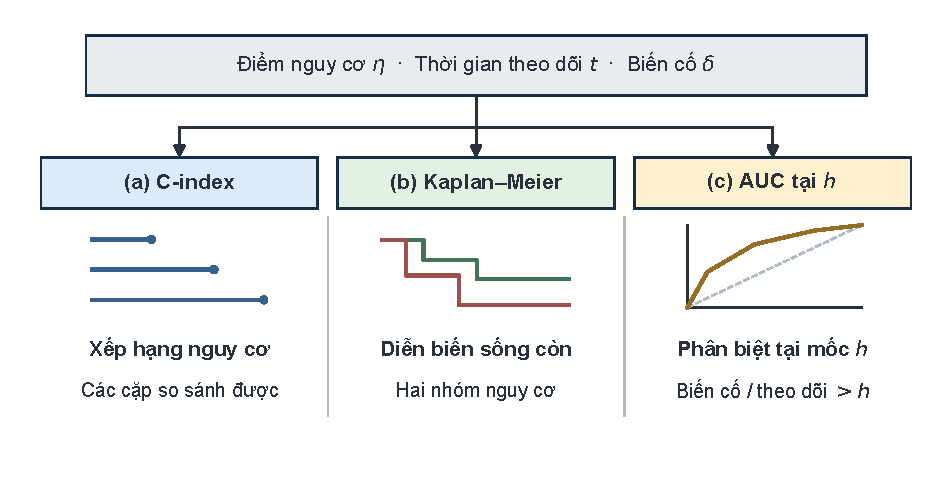
\includegraphics[width=\textwidth]{image/evaluation-map.pdf}
\caption{Ba góc nhìn đánh giá và phân tầng điểm nguy cơ sống còn}
\label{fig:evaluation-map}
\end{figure}

\subsection{C-index}
Chỉ số phù hợp C-index (Concordance Index) theo quy ước Harrell \cite{harrell1996multivariable} là thước đo chuẩn mực nhất để đánh giá năng lực xếp hạng của mô hình sống còn trên toàn bộ dải thời gian theo dõi. Về mặt trực giác, C-index đo lường xác suất mà thứ tự nguy cơ do mô hình dự đoán đồng thuận với thứ tự xảy ra biến cố thực tế giữa hai bệnh nhân bất kỳ.

Cụ thể, xét tất cả các cặp cá thể $(i,j)$ thỏa mãn điều kiện có thể so sánh được: người thứ nhất có biến cố ($\delta_i=1$) và thời điểm biến cố của người đó diễn ra trước thời điểm kết thúc theo dõi của người thứ hai ($t_i<t_j$). Nếu mô hình dự báo chính xác rằng người gặp biến cố sớm hơn có điểm nguy cơ cao hơn ($\eta_i>\eta_j$), cặp đó được chấm 1 điểm đồng thuận. Trường hợp mô hình dự đoán hai người có cùng điểm nguy cơ ($\eta_i=\eta_j$), cặp đó được chấm 0.5 điểm. Ngược lại, nếu thứ tự dự báo bị đảo ngược ($\eta_i<\eta_j$), cặp đó nhận 0 điểm. Các cặp có thời gian theo dõi bằng nhau hoặc cả hai cùng bị kiểm duyệt không thể xác định thứ tự nên không được đưa vào so sánh. C-index bằng 0.5 tương đương với mức đoán ngẫu nhiên, trong khi 1.0 đại diện cho khả năng phân biệt hoàn hảo. Kết quả C-index qua ba lần khởi tạo được báo cáo dưới dạng trung bình $\pm$ độ lệch chuẩn mẫu (SD, mẫu số $n-1$) nhằm phản ánh độ ổn định của kiến trúc trước biến thiên ngẫu nhiên của trọng số ban đầu.

\subsection{Kaplan--Meier và nhóm nguy cơ đồng thuận}
Trong thực hành y khoa, các chỉ số điểm số liên tục cần được chuyển hóa thành các phân tầng nguy cơ rõ ràng để hỗ trợ bác sĩ phân loại bệnh nhân và đưa ra phác đồ theo dõi thích hợp. Để thực hiện việc này một cách hoàn toàn khách quan và không chịu thiên lệch từ tập kiểm tra, tôi sử dụng trung vị của điểm nguy cơ $\eta$ trên tập huấn luyện làm ngưỡng phân nhóm. Người có điểm nguy cơ vượt trên ngưỡng trung vị được xếp vào nhóm nguy cơ cao, trong khi những người có điểm bằng hoặc thấp hơn ngưỡng thuộc nhóm nguy cơ thấp.

Tuy nhiên, việc phân nhóm chỉ dựa trên một mô hình đơn lẻ có thể chịu ảnh hưởng bởi tính ngẫu nhiên của lần khởi tạo đó. Do đó, tôi áp dụng \emph{nguyên tắc đồng thuận đa số} (majority voting): một người tham gia được xếp vào nhóm nguy cơ cao (hoặc thấp) nếu có ít nhất hai trong ba lần khởi tạo cùng phân loại người đó vào nhóm này. 

Sau khi xác lập nhóm đồng thuận, đường cong Kaplan--Meier (KM) \cite{kaplan1958nonparametric} được sử dụng để ước lượng xác suất chưa ghi nhận biến cố suy giảm nhận thức theo thời gian ở từng nhóm. Hai đường cong được trình bày kèm theo dải khoảng tin cậy (CI) 95\%, các dấu kiểm duyệt tại thời điểm rời theo dõi, cùng bảng số lượng người còn nguy cơ (number at risk) ngay trước các mốc 0, 2, 3 và 5 năm. Sự khác biệt giữa hai đường cong được kiểm định chặt chẽ bằng kiểm định log-rank để xác định ý nghĩa thống kê. Đồng thời, một mô hình hồi quy Cox đơn biến được áp dụng trên nhãn phân nhóm để định lượng tỷ số nguy cơ (Hazard Ratio - HR) cùng khoảng tin cậy 95\%, cho biết người thuộc nhóm nguy cơ cao có tốc độ gặp biến cố gấp bao nhiêu lần so với nhóm nguy cơ thấp. Giả định nguy cơ tỷ lệ được kiểm tra cẩn trọng thông qua phần dư Schoenfeld với thời gian được biến đổi theo thứ hạng. Mặc dù đồ thị chỉ thể hiện năm năm đầu nhằm tập trung vào giai đoạn can thiệp sớm, kiểm định log-rank và ước lượng HR sử dụng trọn vẹn toàn bộ thời gian theo dõi.

\subsection{AUC theo thời gian tại 2, 3 và 5 năm}
Bên cạnh khả năng xếp hạng toàn cục của C-index, các bác sĩ thường đối mặt với các câu hỏi tiên lượng cụ thể tại những cửa sổ thời gian xác định: ``Liệu bệnh nhân này có tiến triển trong vòng 2 năm tới hay không? 3 năm? hay 5 năm?''. Để trả lời chính xác câu hỏi này, tôi sử dụng diện tích dưới đường cong ROC phụ thuộc thời gian (time-dependent cumulative/dynamic AUC).

Tại mỗi mốc thời gian đánh giá $h \in \{2, 3, 5\text{ năm}\}$, tập bệnh nhân được phân chia thành hai nhóm: nhóm biến cố $\mathcal C_h=\{i:\delta_i=1,t_i\leq h\}$ gồm những người đã thực sự suy giảm nhận thức trước hoặc tại mốc $h$; và nhóm đối chứng $\mathcal D_h=\{j:t_j>h\}$ gồm những người vẫn duy trì tình trạng ổn định sau mốc $h$. Thách thức toán học lớn nhất ở đây là hiện tượng kiểm duyệt: những người bị kiểm duyệt trước thời điểm $h$ không thể biết chắc chắn tình trạng bệnh lý tại $h$, do đó không thể gán vào nhóm nào. Nếu đơn thuần loại bỏ những người này, mẫu đánh giá sẽ bị sai lệch nghiêm trọng.

Để giải quyết bài toán kiểm duyệt một cách chuẩn xác, tôi áp dụng phương pháp gán trọng số nghịch đảo xác suất kiểm duyệt (Inverse Probability of Censoring Weighting - IPCW) \cite{polsterl2020scikit,hung2010time}. Trọng số IPCW bù đắp xác suất bị mất dấu bằng cách gán trọng số $w_i = 1/\widehat G(t_i)$ cho mỗi ca biến cố quan sát được, trong đó hàm phân phối kiểm duyệt $\widehat G(u)$ được ước lượng từ tập huấn luyện thông qua đường Kaplan--Meier cho biến cố kiểm duyệt. Công thức ước lượng AUC tích lũy/động có dạng:
\begin{equation}
 \widehat{\operatorname{AUC}}(h)=
 \frac{\displaystyle\sum_{i\in\mathcal C_h}w_i
 \sum_{j\in\mathcal D_h}\kappa(\eta_i,\eta_j)}
 {\displaystyle |\mathcal D_h|\sum_{i\in\mathcal C_h}w_i},
 \qquad
 \kappa(a,b)=\begin{cases}
 1,&a>b,\\
 \tfrac12,&a=b,\\
 0,&a<b.
 \end{cases}
 \label{eq:ipcw-auc}
\end{equation}
Ý nghĩa của Công thức~\eqref{eq:ipcw-auc} là tính toán tỷ lệ các cặp (biến cố, đối chứng) mà mô hình xếp hạng đúng, có điều chỉnh trọng số để đại diện cho toàn bộ quần thể ban đầu. Khi triển khai tính toán bằng thư viện \texttt{scikit-survival}, các điểm nguy cơ kề nhau chênh lệch dưới $10^{-8}$ được coi là đồng điểm. Đồng thời, để tránh nguy cơ ngoại suy phân phối kiểm duyệt khi thời gian theo dõi tối đa ở tập xác thực (18.26 năm) vượt quá tập huấn luyện (13.95 năm), quy trình áp dụng kỹ thuật chặn thời gian theo dõi tại ngưỡng $h+\varepsilon$ (với $\varepsilon$ được xác định chính xác qua hàm \texttt{nextafter}). 

Tổng kết lại, bộ ba chỉ số C-index, Kaplan--Meier và IPCW-AUC tạo nên một khung đánh giá toàn diện và khắt khe, kiểm chứng vững chắc năng lực của mô hình RC-Free từ góc độ lý thuyết xếp hạng đến ứng dụng phân tầng nguy cơ thực tiễn trong y khoa. Toàn bộ các kết quả thực nghiệm chi tiết sẽ được trình bày và phân tích có hệ thống trong Chương~\ref{chap:results}.

\FloatBarrier
